\documentclass[11pt,a4paper,openany]{article}
\usepackage[utf8]{inputenc}
\usepackage[spanish,es-tabla]{babel}
\usepackage{csquotes}
\usepackage{listings}
\usepackage{float}
\usepackage{hyperref}
\usepackage{amsmath}
\usepackage{amsfonts}
\usepackage{lmodern}
\usepackage{multirow} 
\usepackage{amssymb}
\usepackage{graphicx}
\usepackage{tikz}
\usepackage{subfigure}
\usepackage{pdflscape}
\usepackage{lipsum}
\usepackage{setspace}
\usepackage[backend=biber,style=apa,sorting=nyt]{biblatex}
\usepackage[left=2.0cm, right=2.0cm, top=2.00cm, bottom=2.00cm]{geometry}
\addbibresource{bibliografia.bib} 



\begin{document}
\pagestyle{plain}

\begin{titlepage}

\begin{picture}(-5,0)(2.5,0)
\put(-40,-735){
\includegraphics[width=100pt,height=50pt]{logo1.png}}
\end{picture}	
    
\begin{tikzpicture}[overlay]
  \path(0pt,0pt);
  \draw[line width=6.5pt,line join=round](30pt, -20pt) -- (380pt, -20pt);
  \draw[line width=3.5pt,line join=round](460pt, -80pt) -- (460pt, -655pt);
\end{tikzpicture}

\begin{picture}(-5,0)(2.5,0)
\put(395,-20){
\includegraphics[width=90.144pt,height=85.4pt]{Tecnm_logo.png}}
\end{picture}

\begin{tikzpicture}[overlay] 
   \path(0pt,0pt);
   \draw[line width=6.5pt,line join=round](470pt, -40pt) -- (470pt, -640pt);
   \draw[line width=3.5pt,line join=round](40pt, -1pt) -- (370pt, -1pt);
\end{tikzpicture}

\begin{picture}(-5,0)(2.5,0)
\put(-40,40){
\includegraphics[width=224.25pt,height=46.24pt]{SEP_logo.png}} 
\end{picture}

    \centering
    \vspace{1.5cm} 

 	{\fontsize{26}{26} \bf Tecnológico Nacional de México}
 	\vspace{0.5cm}

 	{\fontsize{24}{24} Centro Nacional de Investigación y Desarrollo Tecnológico}
 	\vspace{1.5cm}
    
{\fontsize{18}{18} \bf Doctorado en Ciencias en Ingeniería Electrónica}
        \vspace{1.5cm}

	
   {\fontsize{26}{26} \selectfont \bf Propuesta de Tesis}
 	\vspace{1cm}
 	
 	{\fontsize{14}{14}  \bf Diseño de un método de Aprendizaje Profundo para evaluar la respuesta a tratamientos de tumores sólidos en pacientes con cáncer de pulmón, basado en el procesamiento de información de imágenes médicas}
 	\vspace{2cm}
 	
 	
 	{\fontsize{18}{18}  Presentada por }\\
 	{\fontsize{15}{15} \bf M. en C. Randy Guzmán Gómez }
 	\vspace{2cm}
 	
 	{\fontsize{18}{18}  Director de tesis}\\
 	\vspace{0.2cm}
 	{\fontsize{15}{15} \bf Dra. Ma. Guadalupe López López }\\
 	\vspace{0.5cm}
 	{\fontsize{18}{18} Codirector de tesis}\\
 	\vspace{0.2cm}
 	{\fontsize{15}{15}\bf Dr. Víctor Manuel Alvarado Martínez}
 	\vspace{3cm}
	
 	{Cuernavaca, Morelos, México. Junio de 2024 \par}

\end{titlepage}
 	


\newpage

\tableofcontents 

\newpage

\listoffigures
\listoftables

\newpage


\section*{Nomenclatura}

\begin{table}[h]
    \centering
    \caption{Siglas y Acrónimos.}
     \vspace{0.3cm}
    \begin{tabular}{ p{3cm} p{12cm} }
        Siglas & Descripción \\ \hline 
        CPCNP & Cáncer de Pulmón de Células No Pequeñas \\ 
        CPCP & Cáncer de Pulmón de Células Pequeñas \\ 
        TNE & Tumores Neuroendocrinos\\
        CCE & Carcinoma de Células Escamosas\\
        AC & Adenocarcinoma\\
        CCG & Carcinoma de Celulas grandes\\
        RECIST & Response Evaluation Criteria In Solid Tumors \\ 
        EORTC & European Organisation for Research and Treatment of Cancer  \\ 
        OMS & Organización Mundial de la Salud  \\ 
        TC  & Tomografia Computarizada\\ 
        TEP  & Tomografía por Emisión de Positrones\\
        RM  & Resonancia Magnetica \\ 
        IA  & Inteligencia Artificial\\
        DL  & Deep learning (Aprendizaje profundo)\\
        ML  & Machine Learning (Aprendizaje de maquinas)\\
        NN  & Neural Network (Red Neuronal) \\
        ANN  & Artificial Neural Network (Red Neuronal Artificial) \\
        CNN  & Convolutional Neural Network \\ 
        RNN  & Recurrent Neural Network \\ 
    \end{tabular}
\end{table}

\newpage

\section{Introducción}
El cáncer es la principal causa de mortalidad en el mundo. En particular, el carcinoma de pulmón es uno de los tumores más frecuentes y el que más muertes causa (\cite{Xu2019}). Según las estadísticas de la Agencia Internacional para la Investigación sobre el Cáncer (\cite{ferlay_global_2024}), los cánceres con mayor incidencia fueron, en orden descendente: cáncer de mama, pulmón, colorrectal, próstata, piel y cáncer gástrico. Además, se informó que el cáncer de pulmón fue el más letal. De un total de 8,164,372 muertes por cáncer en todo el mundo en 2020, el 22\% se atribuyó al cáncer de pulmón, el 11,45\% al cáncer colorrectal, el 10,17\% al cáncer de hígado, el 9,42\% al cáncer gástrico y el 8,39\% al cáncer de mama.\\
\\
A lo largo de las décadas, se ha desarrollado tratamientos prácticos y de vanguardia para combatir el cáncer. Los tratamientos farmacológicos y de radiación para el cáncer incluyen la quimioterapia y la radioterapia. La cirugía también es una opción para combatir esta enfermedad. Sin embargo, la tasa de supervivencia global de los pacientes con cáncer de pulmón es de cinco años como máximo en algunos casos (\cite{Bianconi2020}). En vista de esto, también se han concebido métodos de seguimiento para evaluar la respuesta del paciente a estos tratamientos. Sin embargo, el progreso del tratamiento y los mecanismos de seguimiento presentan desafíos. La valoración de los tratamientos debe mejorarse en precisión y velocidad para conocer la respuesta del tumor y actuar a su debido tiempo. Esto, a su vez, evitará la toxicidad y la pérdida de tiempo al dispensar tratamientos que no son adecuados para los pacientes. Actualmente, existen dos formas estándar de monitorear las respuestas terapéuticas. El primer método encuentra cambios morfológicos y sigue detalles anatómicos a través de la tomografía computarizada (TC), que escanea la estructura interna del cuerpo. La segunda forma es discernir cambios metabólicos mediante tomografía por emisión de positrones (PET) (\cite{Shang2016}). Ambos métodos ayudan a evaluar la respuesta del tumor al tratamiento y guían acciones posteriores.\\

La inteligencia artificial (IA) ha surgido como una fuerza transformadora en varios campos y ha impulsado cambios en la práctica médica. La integración del aprendizaje automático (ML) y el aprendizaje profundo (DL), dos ramas de la IA, en los métodos de radiología es una tendencia. Esta fusión facilita el camino para una extracción más especializada de datos cuantitativos de imágenes y promete un futuro para un diagnóstico y tratamiento de enfermedades más efectivos. De hecho, las imágenes médicas y las herramientas computacionales se unen en un término que se encuentra con frecuencia en la literatura como radiómica (\cite{Lambin2017}). Este campo utiliza herramientas de IA para extraer conocimiento intrínseco de imágenes o datos médicos. Es un método que brinda información a los especialistas sobre la intensidad, forma, tamaño, volumen o estructura de los tejidos. Por ejemplo, medir estas variables es vital en el tratamiento y seguimiento del cáncer. Por lo tanto, el enfoque radiómico es una forma práctica de abordar el desafío crítico de la cura del cáncer. En este contexto, una de las principales causas de muerte en todo el mundo tanto en hombres como en mujeres es el cáncer de pulmón de células no pequeñas (CPCNP). El presente estudio bibliográfico se centra en la valoración de las respuestas de los pacientes a los tratamientos del cáncer de pulmón. \\

El documento se organiza de la siguiente manera: en la Sección 2, damos una descripción general de los tipos de cáncer de pulmón de células no pequeñas y las técnicas de imagen más utilizadas en oncología. Luego, recapitulamos los criterios de respuesta estándar para la evaluación del tratamiento del cáncer de pulmón y cómo se aplican en la evaluación clínica. Después, continuamos con una descripción de los modelos de aprendizaje profundo utilizados para el procesamiento de imágenes y las métricas para evaluar el rendimiento de las redes neuronales. En la Sección 3, presentamos los trabajos de investigación más relevantes centrados desde la evaluación clínica del cáncer de pulmón hasta la aplicación de métodos de DL aplicados al diagnostico y la evaluación de tratamientos. Finalmente, en la Sección 4, discutimos la propuesta de investigación que va desde la descripción del problema hasta la metodología necesaria para cumplir los objetivos y el cronograma de actividades planteado.

\section{Marco conceptual}
    \subsection{Radiología}
    La radiología es una rama de la medicina que utiliza imágenes para el diagnóstico y tratamiento de lesiones y enfermedades. Las técnicas de generación de imágenes que utiliza la radiología han sido posible gracias a la evolución experimentada en el campo de la microelectrónica que ha facilitado el desarrollo de nuevos y mejores sistemas de detección digital de la imagen (\cite{Silva2019}).
    
        \subsubsection{Estudios de imagen para cáncer de pulmón}
        Los principales tipos histológicos de cáncer de pulmón son el cáncer de pulmón de células no pequeñas (CPCP), el carcinoma de pulmón de células pequeñas (CPCNP) y los tumores neuroendocrinos (TNE). El tipo de CPCNP se clasifica además en carcinoma de células escamosas (CCE), adenocarcinoma (AC) y carcinoma de células grandes (CCL) (\cite{ambrosini_petct_2012}). \\
        \\
        En oncología, las imágenes son esenciales en la detección, el diagnóstico, el seguimiento del tratamiento y el pronóstico del cáncer. Las técnicas de imagen anatómica estándar para la estadificación y reestadificación en pacientes con CPCNP son la radiografía de tórax, la ecografía, la tomografía computarizada (TC), la resonancia magnética (RM) y los estudios que se basan en la medicina nuclear. Además, las tecnologías están desempeñando un papel en la medicina nuclear. La tomografía por emisión de positrones (PET) ha evolucionado hasta convertirse en una prueba de rutina para controlar los tumores sólidos, incluido el cáncer de pulmón (\cite{ambrosini_petct_2012}).\\
        
        \noindent{\textbf{Tomografía computarizada:}}\\
        La TC es una técnica derivada de la obtención de imágenes por rayos X y ha sido mejorada por la tecnología informática. Las exploraciones obtenidas son imágenes tridimensionales de cualquier región anatómica. La función de una tomografía computarizada es medir la transmisión de rayos X a través del paciente en múltiples proyecciones. Las proyecciones son producidas por el tubo de rayos X que gira alrededor del paciente. La computadora de la máquina procesa las señales recibidas para generar imágenes transversales o "cortes". Los cortes sucesivos se pueden "apilar" digitalmente para formar una imagen tridimensional del paciente que permite identificar las estructuras internas básicas \cite{Calzado2010}.\\

        \noindent{\textbf{Tomografía por emisión de positrones:}}\\
        La PET es una técnica de obtención de imágenes en medicina nuclear similar a una TC. Una diferencia clave es que la PET necesita que se inyecten radiofármacos en el torrente sanguíneo del paciente. Como resultado, se adquieren imágenes de los procesos bioquímicos internos. Esta técnica permite medir el consumo regional de glucosa y cuantificar la actividad metabólica \cite{Guaman2024}.\\
        Los biomarcadores de las imágenes estructurales y funcionales pueden coincidir en los detalles que proporcionan, pero algunos datos son distintivos de cada método. La PET puede detectar anomalías funcionales antes de que puedan ser percibidas por las imágenes estructurales establecidas. Esta modalidad de obtención de imágenes se considera el estándar de oro para la detección del cáncer. Sin embargo, es una técnica invasiva y, al igual que con otras modalidades de imágenes médicas, su interpretación puede ser subjetiva. \\

        Está bien establecido que la TC ha sido el método de imagen estándar más importante para la estadificación del CPCNP. Las TC pueden permitir una medición precisa del tamaño del tumor. Por otro lado, la PET es factible y más precisa para diagnostico. En este contexto, las imágenes funcionales y las técnicas mixtas tienen un papel cada vez mayor en el control del CPCNP. Se ha introducido una tomografía PET/TC combinada para producir imágenes más precisas. También se han desarrollado enfoques de aprendizaje profundo para la detección del cáncer de pulmón sobre tomografías PET/TC combinadas. Las aplicaciones incluyen la diferenciación de nódulos benignos y tumores sólidos pulmonares.\\

        
    \subsection{Criterios de evaluación para cáncer de pulmón}\label{Section:TEM}
    Los escáneres médicos proporcionan un paquete de múltiples imágenes transversales de los órganos internos de los pacientes. Estas imágenes son bidimensionales y se construyen en cortes. Por lo tanto, la fusión de cortes permite una visión volumétrica del órgano. Antes de la interpretación, se debe evaluar el conjunto de datos 2D o 3D de los escáneres para interpretar las anomalías y el cáncer del paciente. Después de la adquisición de la imagen, el primer paso de este proceso es seleccionar el intervalo de corte. En ese sentido, el radiólogo enmarca la región de estudio. Según el tipo de tecnología de escaneo, esta decisión se toma de manera diferente. Esta revisión trata sobre dos enfoques estándar para sentar las bases para la evaluación de tumores. Estos se describen en términos generales en la Fig.~\ref{fig:TOE}.

    \begin{figure}[H]
    \centering
    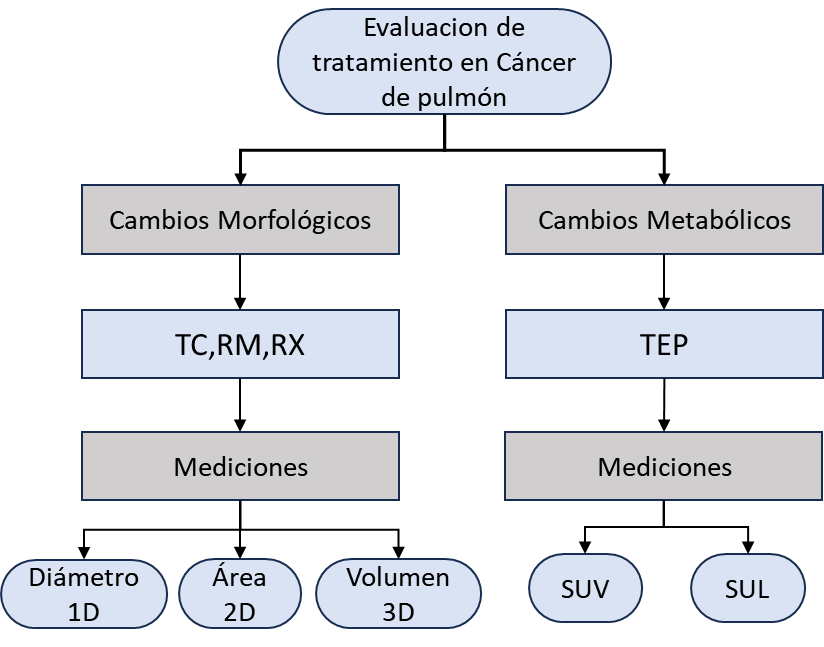
\includegraphics[width=9cm]{TypeofEvaluation-Diagram.png}
    \caption{Tipos de mediciones utilizadas en la evaluación de tratamientos de CPNM\label{fig:TOE}}
    \end{figure}

    En el seguimiento de un tratamiento de CPCNP, las pruebas de imagen por TC muestran la evolución morfológica de las lesiones del paciente. En cambio, las imágenes PET revelan cambios metabólicos. Las pruebas de lesiones pulmonares guiadas por estos medios se realizan antes y después del tratamiento para permitir la medición de los cambios en las lesiones. Los ensayos clínicos han utilizado diversos criterios para evaluar la respuesta al tratamiento del cáncer. Sin embargo, se han realizado esfuerzos para estandarizar esta evaluación. Hoy en día, los estándares se han implementado con éxito en la práctica médica y continúan desarrollándose. El diámetro, el área o el volumen de las lesiones son las medidas viables que se pueden obtener a partir de las imágenes de TC. Por otro lado, el volumen de absorción de un radiofármaco es la medida a tratar en las imágenes PET. Más precisamente, los indicadores cuantitativos para caracterizar la lesión en las exploraciones PET son el Valor de captación estandarizado (SUV) y la captación estándar en función de la masa corporal magra (SUL) (Fig.~\ref{fig:TOE}). \\

    
        \subsubsection{Criterios basados en cambios morfológicos}\label{seccion:CBMC}
         El objetivo fundamental del seguimiento del tratamiento del cáncer consiste en comparar las exploraciones por imágenes previas y posteriores al tratamiento. Finaliza con la aplicación de los criterios de evaluación. RECIST, es la guía estándar a nivel mundial para determinar la eficacia del tratamiento o la terapia. El procesamiento global de las imágenes comienza con la elección de las "lesiones objetivo". Estas lesiones tumorales siguen siendo el objeto de estudio durante los seguimientos de la enfermedad. La lesión objetivo debe elegirse en función de su variabilidad, la dificultad de medición y después de la especificación del intervalo de corte en las imágenes de TC (\cite{Deval2014}). RECIST define cuatro criterios principales para la evaluación de las lesiones objetivo. Otros criterios comprenden tres posibles respuestas en lesiones no objetivo (véase la tabla \ref{tab:RECISTRESPONSES}). Cabe destacar que el éxito en la evaluación de la respuesta parcial resuelve la eficacia de la evaluación de la respuesta general al tratamiento del cáncer (\cite{Eisenhauer2009}).

            \begin{table}[h]
                \caption{Evaluación de las lesiones según RECIST.\label{tab:RECISTRESPONSES}}
                \begin{tabular}{p{3cm} p{5cm} p{7cm}}
                    \hline
                    \textbf{Tipo de lesión} & \textbf{Criterios de respuesta} & \textbf{Condición} \\\hline
                    \multirow{4}{*}{Lesión objetivo} & Respuesta completa (CR) & Desaparición de todas las lesiones objetivo o cualquier ganglio linfático patológico. \\
                    & Respuesta parcial (PR) & Al menos una disminución del 30\% en la suma de los diámetros de la lesión objetivo. \\
                    & Enfermedad progresiva (PD) & Al menos un aumento del 20\% en la suma de los diámetros de la lesión diana y demostrar un aumento absoluto de al menos 5 mm. La aparición de una o más lesiones nuevas también se considera progresión. \\
                    & Enfermedad estable (ED) & Sin contracción o aumento suficiente para calificar como PR o ED. \\\hline
                    \multirow{3}{*}{Lesión no objetivo} & Respuesta completa (RC) & Desaparición de todas las lesiones no objetivo. \\
                    & Enfermedad progresiva (EP) & Progresión inequívoca de lesiones no objetivo existentes. La aparición de una o más lesiones nuevas se considera progresión.\\
                    & Enfermedad estable (ED) & Persistencia de una o más lesiones no objetivo.\\      
                    \hline
                \end{tabular}
            \end{table}

        
        \subsubsection{Criterios basados en cambios metabólicos}
        Durante la exploración PET en la detección del cáncer, se administran al paciente por vía intravenosa trazadores que imitan la glucosa, como la fluorodesoxiglucosa (FDG). Las imágenes PET capturan los diferentes niveles de concentración de FDG en los tumores, cuantificados por el nivel de SUV. Como la progresión y la destrucción del tumor se correlacionan con este nivel, es un excelente índice para medir la actividad tumoral. Actualmente, la respuesta al tratamiento del cáncer se puede estudiar en imágenes PET a través de dos criterios opcionales. La Organización Europea para la Investigación y el Tratamiento del Cáncer (EORTC) desarrolló en 1999 el primer conjunto de criterios. El segundo son los Criterios de Respuesta PET en Tumores Sólidos (PERCIST), introducidos en 2009 (\cite{Kim2016}). Se trata de enfoques bastante diferentes. Los criterios de la EORTC ayudan a evaluar las regiones de interés (ROI) de lesiones específicas elegidas en el punto de partida y monitoreadas en cada exploración posterior. A partir de ahora, el SUV se corrige en función de la superficie corporal. Luego, para cada exploración PET, el SUV se calcula en función de la masa corporal (SUL). Se realiza para un volumen de ROI que satisface un diámetro máximo de 12 mm. Por otro lado, en la práctica clínica, PERCIST se considera un método más sencillo de aplicar, ya que proporciona más detalles sobre cómo definir las lesiones diana (\cite{Skougaard2013}). Las respuestas metabólicas de los tumores según ambos criterios se muestran en la Tabla \ref{tab:SUVRESPONSES}.

        \begin{table}[h]
            \caption{Evaluación de las lesiones según EORTC y PERCIST.\label{tab:SUVRESPONSES}}
            \begin{tabular}{p{4cm} p{5.4cm} p{5.4cm}}
                \hline
                \textbf{Criterio de respuesta} & \textbf{EORTC} & \textbf{PERCIST} \\
                \hline
                \multirow[m]{3}{*}{}Respuesta metabólica completa (CMR) & Resolución completa de la captación de FDG en todas las lesiones. & Resolución completa de la captación de FDG en todas las lesiones.\\
                \hline
                \multirow[m]{3}{*}{}Respuesta metabólica parcial (PMR) & Reducción mayor del 25\% en la suma de SUVmax después de más de un ciclo de tratamiento. & Una reducción mínima del 30\% del SUV de masa corporal magra máxima (SULpeak) y una caída absoluta de 0,8 unidades de SULpeak.\\
                \hline
                \multirow[m]{3}{*}{}Enfermedad metabólica progresiva (PMD) & Más del 25\% de aumento en la suma de SUVmax o aparición de nuevas lesiones ávidas de FDG. & Más del 30\% de aumento en el SULpeak de la captación de FDG y un aumento absoluto de 0,8 SULpeak, o aparición de nuevas lesiones ávidas de FDG.\\
                \hline
                \multirow[m]{3}{*} {}Enfermedad estable (SD)& No califica para CMR, PMR o PMD. & No califica para CMR, PMR o PMD.\\
                \hline
                \end{tabular}       
        \end{table}
        
    \subsection{Radiomica}
    \subsection{Inteligencia artificial}
    La IA combina hardware, software y matemáticas en sistemas informáticos que procesan información emulando acciones o funciones humanas. La IA utiliza el razonamiento lógico para resolver problemas simples o para concebir sistemas expertos de toma de decisiones. Además, la IA permite que los sistemas que manejan grandes cantidades de datos aprendan y resuelvan problemas. El ML es una rama de la IA que permite que las computadoras aprendan. En esta secuencia, el DL es una forma de ML que utiliza algoritmos para automatizar tareas. Expresamente, los recursos de DL se planifican y construyen en redes neuronales profundas, donde los datos de entrada se analizan en diferentes capas (\cite{wang_deep_2022}). \\ 
        
    \subsection{Redes neuronales profundas}

    Para entender como se compone una red neuronal profunda , debemos analizar el modelo del perceptrón. Un perceptrón es una función matemática que se basa en un modelo neuronal biológico y es indispensable para las redes neuronales artificiales (ANN) de DL. El perceptrón recibe las señales de entrada. Si la suma de las señales supera un umbral determinado, se produce una señal de salida. En el marco del ML, es lo que permite predecir la categoría de una muestra de datos. asociando el valor de salida a una clase determinada, por tanto, se trata de un elemento esencial (\cite{P_ADELI_1989}). En la Fig.~\ref{fig:Perceptron}, se muestra la representación gráfica de una Neurona artificial (Perceptrón).

    \begin{figure}[h]
            \centering
            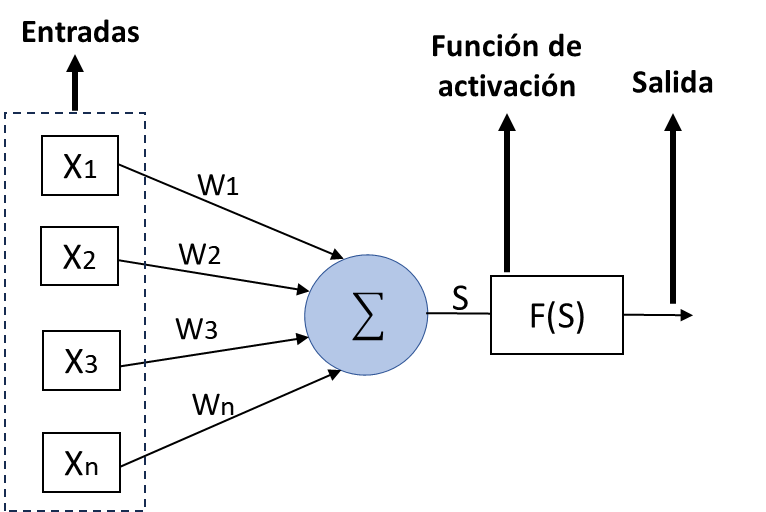
\includegraphics[width=6cm]{Perceptron.png}
            \caption {Perceptrón. \label{fig:perceptron}}
        \end{figure}

    Los datos de entrada \textbf{X} se multiplican por los coeficientes de peso \textbf{W}. El resultado es un valor.\\
    \\
    Ese valor puede ser positivo o negativo. Y sirve como entrada para la función de activación. Si el peso calculado de los datos de entrada supera un umbral determinado se entrega el valor de salida. \\
    \\
    El resultado predicho se compara con el resultado conocido. En caso de diferencia, el error se retropropaga para permitir ajustar los pesos. Al combinar múltiples neuronas artificiales por capas, generamos lo que se conoce como redes neuronales profundas, y estas redes ofrecen una potencia de cálculo superior para aproximar modelos mas complejos. En la Fig.~\ref{Fig:ANN} anexo A, se muestra la representación gráfica de una red neuronal artificial multicapa.\\

    Varios tipos de redes neuronales con diversos objetivos de tratamiento de imágenes han surgido como activos valiosos en diferentes campos, incluida la industria de la salud (\cite{Shahid2019}). Las arquitecturas populares para redes de aprendizaje profundo se enumeran en la Tabla \ref{tab:DLN}, con una breve descripción de su objetivo de aplicación.\\

    \begin{table}[H]
        \caption{Resumen de las redes DL.\label{tab:DLN}}
        \begin{tabular}{l p{8cm} l}
        \hline
        \bf{Red DL} & \bf{Aplicaciones principales} & \bf{Referencia} \\
        \hline
        CNN & Procesamiento de imágenes (detección, modelado, segmentación) & \cite{Lecun1989} \\
        \hline
        RNN & Análisis de series temporales, Procesamiento del lenguaje (Modelado, análisis, traducción) y Reconocimiento de voz & \cite{Cho2014} \\
        \hline
        RvNN & Análisis de estructura molecular y Procesamiento del lenguaje (Modelado estadístico, análisis) & \cite{Goller1996} \\
        \hline
        DBN & Reconocimiento de imágenes, reconocimiento de voz y procesamiento del lenguaje natural & \cite{Hinton2009} \\
        \hline
        DBM & Imágenes Reconocimiento y reconocimiento de voz & \cite{Salakhutdinov2009} \\
        \hline
        GAN & Genera imágenes, completa la información faltante y genera modelos 3D a partir de datos 2D & \cite{Goodfellow2014} \\
        \hline
        VAE & Genera nuevos datos & \cite{kingma2013,Singh2021} \\
        \hline
        \end{tabular}
        \begin{tabular}{l}
        \footnotesize CNN: Red neuronal convolucional \\
        \footnotesize RNN: Red neuronal recurrente \\
        \footnotesize RvNN: Red neuronal recursiva \\
        \footnotesize DBN: Red de creencias profundas \\
        \footnotesize DBM: Máquinas de Boltzmann profundas \\
        \footnotesize GAN: Red generativa antagónica \\
        \footnotesize VAE: Autocodificador variacional \\
        \end{tabular}
    \end{table}
    
        \subsubsection{Redes neuronales convolucionales}
        Entre las estructuras de DL más utilizadas se encuentran las redes neuronales convolucionales (CNN). Este modelo, introducido por \cite{Lecun1989}, ha logrado un éxito notable. El modelo CNN consta de tres capas: la capa convolucional, la capa de agrupamiento y la capa completamente conectada. La capa convolucional es una operación matemática donde la suma ponderada de los píxeles vecinos calcula el valor de un píxel de salida. La convolución se realiza entre la imagen y una matriz llamada núcleo de convolución (\cite{Esqueda2005}). Como se muestra en la Fig.~\ref{Fig:Conv}. \\

        \begin{figure}[H]
            \centering
            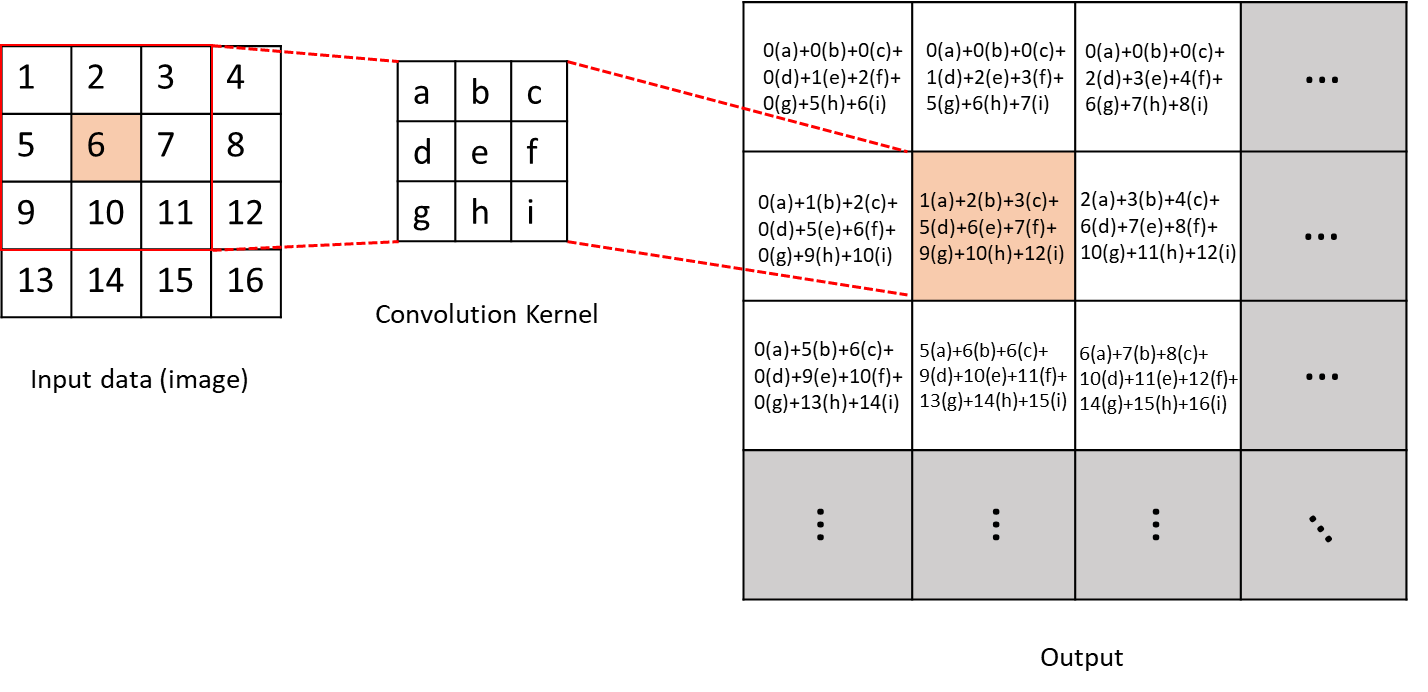
\includegraphics[scale=0.4]{CV.png} 
            \caption{Diagrama esquemático de la operación de convolución. \label{Fig:Conv}}
        \end{figure}

        Las capas de agrupamiento reducen la matriz de la imagen al preservar los píxeles con más información (agrupamiento máximo) o al promediar los píxeles vecinos (agrupamiento medio), como se muestra en la Fig.~\ref{Fig:pool}, anexo B. \\

        Luego, la tarea de clasificación se puede realizar a través de una capa completamente conectada en la etapa final (\cite{Manakitsa2024}). CNN se destaca en la extracción de características y ha establecido firmemente su dominio en el reconocimiento de imágenes para la clasificación. La Fig.~\ref{fig:CNN-A} muestra un ejemplo de la estructura de CNN.
    
        \begin{figure}[h]
            \centering
            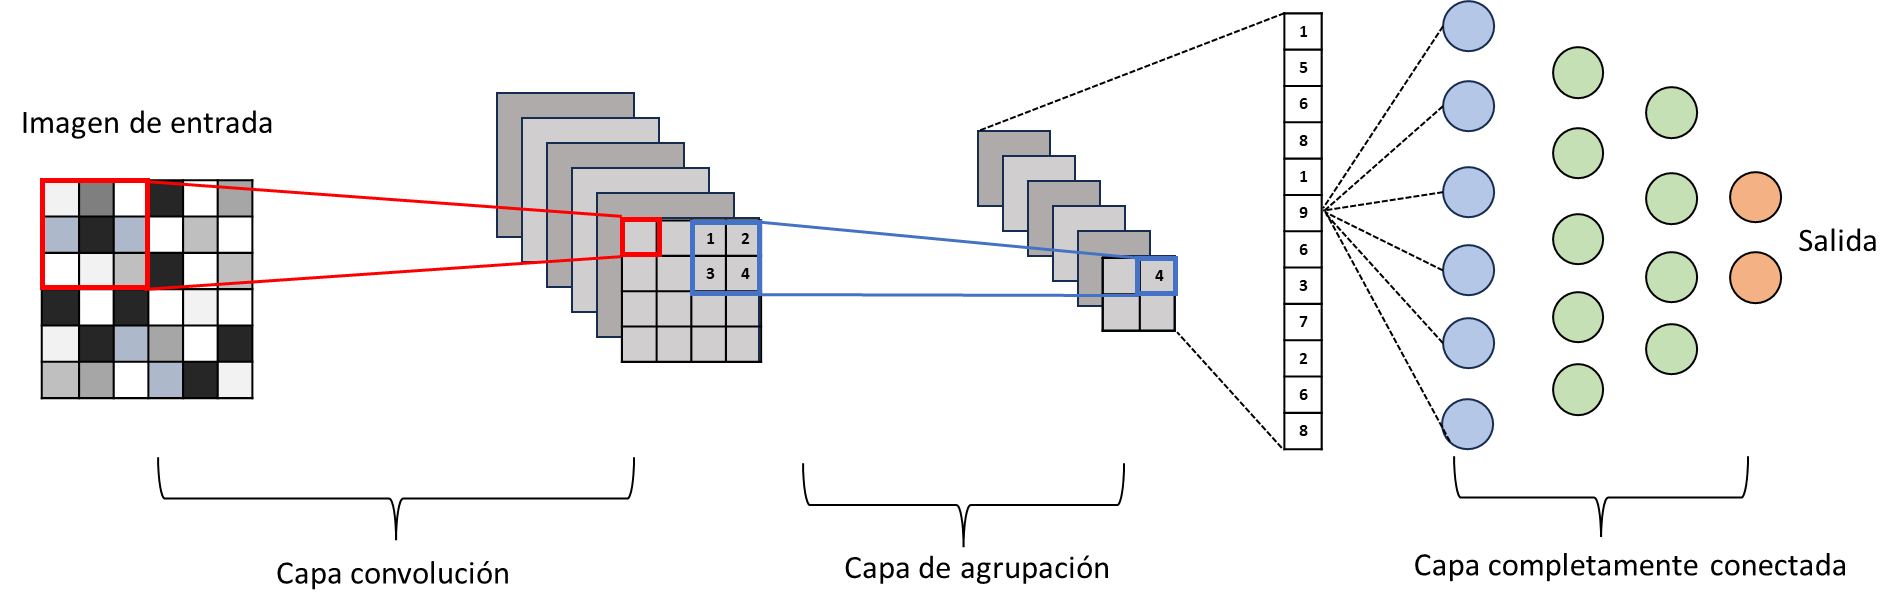
\includegraphics[width=13cm]{CNN.png}
            \caption {Arquitectura general CNN. \label{fig:CNN-A}}
        \end{figure}


        \noindent{\textbf{U-Net}}\\
        
        Una arquitectura CNN ampliamente utilizada para realizar tareas de segmentación es U-Net, que se introdujo por primera vez por \cite{Ronneberger2015}. El objetivo principal de esta arquitectura era abordar el desafío de los datos anotados limitados en el campo médico. La arquitectura U-Net consta de una ruta de contracción y una ruta de expansión (\cite{Yin2023}). La ruta de contracción contiene capas de convolución y agrupación que extraen información contextual y reducen la muestra de la entrada, mientras que la ruta de expansión contiene capas de deconvolución que decodifican los datos extraídos y utilizan la información de la ruta de contracción a través de conexiones de salto para generar un mapa de segmentación como se muestra en la Fig.\ref{fig:A-Unet}.

        \begin{figure}[H]
            \centering
            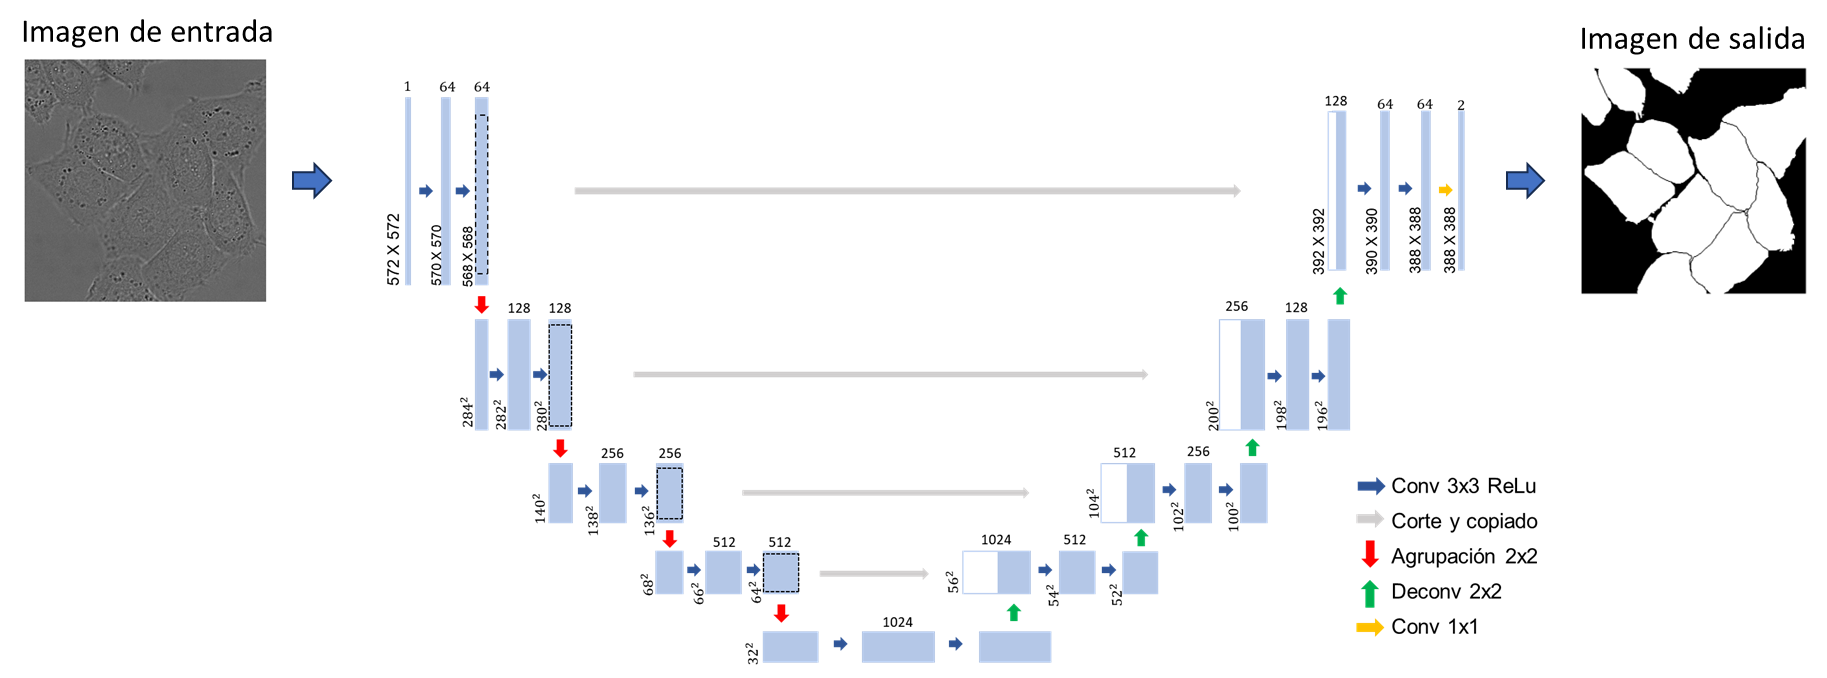
\includegraphics[width=0.7\linewidth]{Unet.png}
            \caption{Arquitectura CNN U-Net.}
            \label{fig:A-Unet}
        \end{figure}
        
        \subsubsection{Redes neuronales recurrentes}

        De manera similar, las redes neuronales recurrentes (RNN) se aplican ampliamente en arquitecturas de aprendizaje automático. Estas redes son modelos de aprendizaje adecuados para procesar datos secuenciales, como el reconocimiento de voz y el procesamiento del lenguaje. Aprenden características de datos de series temporales a través de la memoria de entradas anteriores en el estado interno de la red neuronal. Es decir, la información pasada se almacena implícitamente en la capa oculta y la salida para la entrada actual se calcula considerando todas las entradas anteriores utilizando estos vectores de estado, como se muestra en la Fig.~\ref{fig:RNN-A}. Además, las RNN pueden predecir información futura en función de datos pasados y presentes (\cite{Yu2022}).

        \begin{figure}[H]
            \centering
            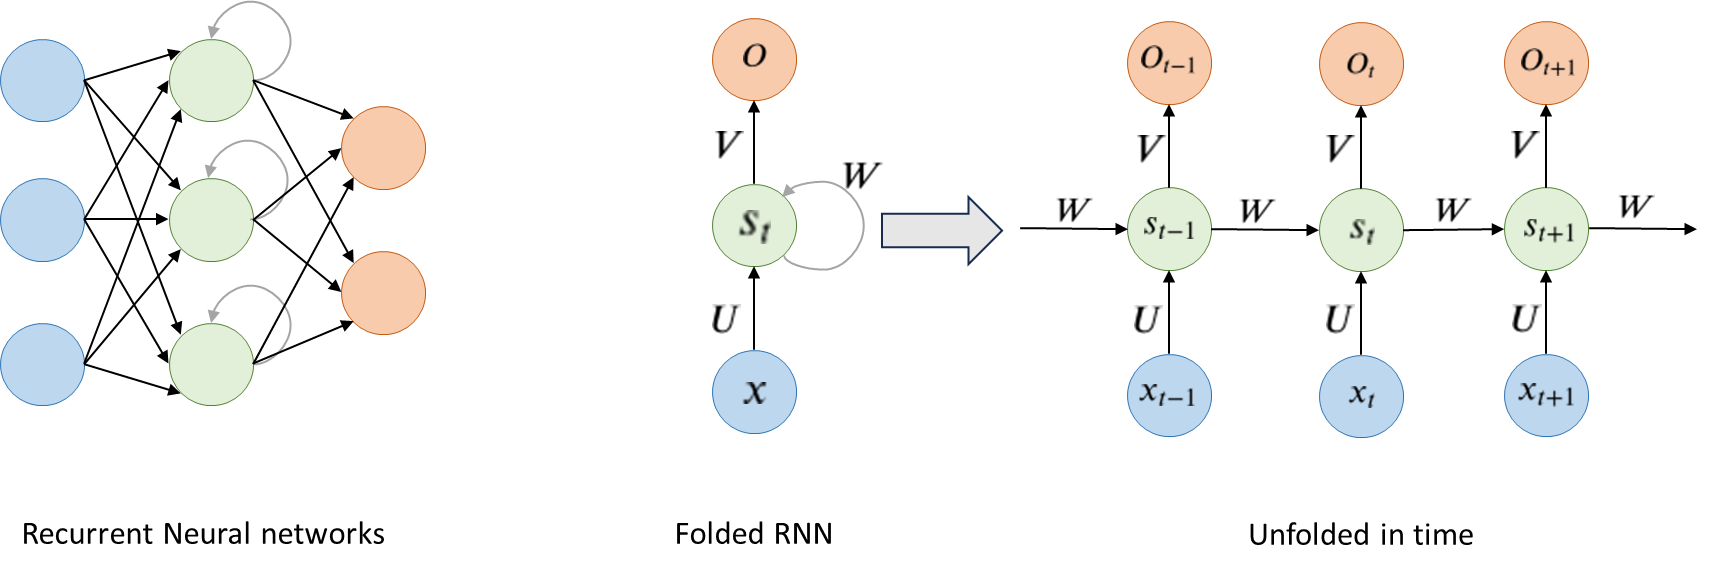
\includegraphics[width=10 cm]{RNN.png}
            \caption {Arquitectura general de RNN \label{fig:RNN-A}}
        \end{figure}

        Como se muestra en la Fig.~\ref{fig:RNN-A}, $x_t$ es la entrada de la secuencia en el tiempo $t$. $s_t$ es la unidad de memoria de la secuencia en el tiempo $t$ y almacena en caché la información anterior, que se calcula mediante la ecuación \ref{EC:SEC}.

        \begin{equation}
            s_t= tanh(\textit{U} x_{t}+ \textit{W} s_{t-1})
            \label{EC:SEC}
        \end{equation}

        $O_t$ es la salida de la capa oculta de la secuencia en el tiempo $t$. Después de pasar por múltiples capas ocultas, se puede obtener la salida final de la secuencia en el tiempo $t$ (\cite{Rajaram2018}).

        \begin{equation}
            O_t= tanh(\textit{V} s_{t})
            \label{EC:OUT}
        \end{equation}
        
        
        
        \subsubsection{Funciones de activación para redes neuronales}
        En el entrenamiento de redes neuronales (NN), la función de activación introduce las no linealidades que hacen que los modelos aprendan funciones complejas (\cite{sharma2017}). Desde los primeros tiempos de las redes neuronales, se han propuesto y probado diferentes versiones de estas funciones. La causa es que las NN aprenden en base a un algoritmo de retropropagación. A continuación, se presentan algunas de las funciones de activación más utilizadas.\\

        La función de activación \textit{Sigmoid} traduce el rango de entrada de $(- \infty; + \infty)$ al rango en $(0; 1)$. Debido al rango de salida de la sigmoide, se satura en 0 o 1, y la salida de cada unidad también se aplasta. Eso significa que el gradiente está alrededor de cero, es decir, se desvanece. Este comportamiento hace que la red sea muy difícil de optimizar después de cierto punto (\cite{Szandaa2020}). La función Sigmoid se expresa en la Tabla \ref{tab:Act-F} y su panorama de salida se muestra en la Fig.~\ref{fig:plotSIG-TANG-ReLU-ELU}, anexo A. \\

        La función \textit{Tangente hiperbólica} tiene una estructura similar a la función Sigmoid. Sin embargo, la función aplasta el valor de entrada en el rango $(-1, + 1)$. La principal diferencia con la función sigmoidea es que su derivada es más pronunciada. Sin embargo, debido a su valor de salida acotado (Fig.~\ref{fig:plotSIG-TANG-ReLU-ELU}, anexo A.) el gradiente también tiende a desaparecer con esta función (\cite{Rasamoelina2020}). Se define en la Tabla \ref{tab:Act-F}.\\

        La función \textit{ReLU} (\textit{Unidad lineal rectificada}) es la función de activación más utilizada en la investigación de aprendizaje profundo por su simplicidad, lo que se traduce en una menor demanda computacional (\cite{Bingham2022}). La función ReLU se expresa en la Tabla \ref{tab:Act-F}. Su salida varía de 0 a infinito. Puede generar un valor cero verdadero, lo que permite la activación de capas ocultas en redes neuronales. La principal desventaja de ReLU es que todos los valores negativos se transforman en cero. Este problema es un caso particular del problema del gradiente evanescente. Por lo tanto, una vez que la neurona se vuelve negativa, es poco probable que se recupere (\cite{glorot2011}). El panorama de salida de la función ReLU se muestra en la Fig. \ref{fig:plotSIG-TANG-ReLU-ELU}, anexo A.\\

        La función \textit{Unidad lineal exponencial} (\textit{ELU}) se propuso por primera vez como una mejora de ReLU en (\cite{clevert2015}), con resultados de clasificación más altos que ReLU tradicional. Para $x \geq 0$, sigue la misma regla que ReLU, y para $x < 0$, aumenta exponencialmente, como se muestra en la Fig.~\ref{fig:plotSIG-TANG-ReLU-ELU}, anexo A. La principal mejora de ELU sobre ReLU es la propiedad de que puede generar valores negativos. La función de activación de ELU se define en la Tabla \ref{tab:Act-F}.\\

        \begin{table}[H]
            \caption{Funciones de activación. (a)Sigmoide, (b) Tangente hiperbólica, (c) Unidad lineal rectificada, (d) Unidad lineal exponencial.\label{tab:Act-F}}
            \centering
            \begin{tabular}{| c | c |}
            \hline
            & \\
            $\sigma(x)=\frac{1}{1+e^{-x}}$ & $ \tanh (x)=\frac{2}{1+e^{-2 x}}-1$ \\
            & \\
            (a) & (b) \\\hline
            & \\
            $\operatorname{ReLU}(x)=\max (0, x)$ & $\operatorname{ELU}(x)=\max (0, x)+\min \left(0, 1\left(e^{x}-1\right)\right)$ \\
            & \\
            (c) & (d) \\\hline
            \end{tabular}
        \end{table}

                
        \subsubsection{Métricas de evaluación}\label{sec:2.5.6}
        Al diseñar métodos de DL para clasificacion o segmentación, se utilizan diferentes métricas para evaluar el rendimiento del modelo, como la especificidad (SPE), la sensibilidad (SEN), la precisión (ACC) y el coeficiente Dice (DC). Estas métricas tienen como objetivo puntuar la similitud entre la salida predicha (o automática) y la salida deseada (o de verdad fundamental) (\cite{Hu2020}). La forma de comparar estas características se basa en el cálculo de una matriz de confusión, en la tabla \ref{tab:confusion_matrix} se muestra un ejemplo de matriz de confusión diseñada para evaluar una segmentación de tejido. Para una tarea de segmentación, se comparan cada uno de los pixeles de la imagen de salida con cada pixel de la verdad fundamental. Para una clasificación de clases, se compara la salida de clasificación con la salida deseada "verdad fundamental". Los elementos de la matriz son el tipo de predicción y los números de ocurrencia asociados (TP, FP, FN y TN) (\cite{Muller2022}). \\

        \begin{table}[H]
        \caption{Matriz de confusión}
            \label{tab:confusion_matrix}
            \centering
            \begin{tabular}{llcc}
            & & \multicolumn{2}{c}{\textbf{Verdad fundamental}} \\ \cline{3-4}
            & \multicolumn{1}{l|}{} & \multicolumn{1}{l|}{Unidades de tejido (1)} & \multicolumn{1}{l|}{Fondo (0)} \\ \cline{2-4}
            \multicolumn{1}{c|}{\multirow{2}{*}{\textbf{Predicción}}} & \multicolumn{1}{l|}{Unidades de tejido (1)} & \multicolumn{1}{c|}{TP} & \multicolumn{1}{c|}{FP} \\ \cline{2-4}
            \multicolumn{1}{c|}{} & \multicolumn{1}{l|}{Fondo (0)} & \multicolumn{1}{c|}{FN} & \multicolumn{1}{c|}{TN} \\ \cline{2-4}
            \end{tabular}\vspace{0.2cm}
            
            \begin{tabular}{l}
            \footnotesize{Nota:}
            \end{tabular}
            \begin{minipage}{11cm}
            \footnotesize{TP: número de píxeles de tejido clasificados correctamente como tejido.} \\
            \footnotesize{FN: número de píxeles de tejido clasificados incorrectamente como fondo.} \\
            \footnotesize{FP: número de píxeles de fondo clasificados incorrectamente como tejido.}\\
            \footnotesize{TN: número de píxeles de fondo clasificados correctamente como fondo.}
            \end{minipage}
        \end{table}


        La especificidad (SPE) calcula la cantidad de negativos reales detectados correctamente.

        \begin{equation}\label{EC:SPE}
            SPE=\frac{TP}{TP+FP}
        \end{equation}

        La sensibilidad (SEN) calcula la cantidad de positivos reales detectados correctamente.

        \begin{equation} \label{EC:SEN}
            SEN=\frac{TP}{TP+FN}
        \end{equation}

        El puntaje de precisión (ACC) es la cantidad de predicciones correctas igual a las predicciones positivas correctas más las predicciones negativas, dividido por la cantidad total de predicciones.

        \begin{equation} \label{EC:ACC}
            ACC=\frac{TP+TN}{TP+TN+FN+FP}
        \end{equation}

        El coeficiente de Dice (DC) mide la similitud entre las regiones segmentadas en forma automática y manual. Se define en (\ref{EC:SEGC})

        \begin{equation} \label{EC:SEGC}
            DC= 2 \times \frac{\left|R_{p} \cap R_{T}\right|}{\left|A_{p}\right|+\left|A_{T}\right|}
        \end{equation}

        donde $R_p$ significa la región de segmentación automática y $R_T$ es la región de verdad fundamental. $A_{p}$ es el número de píxeles de la región de segmentación automática y $A_{T}$ es el número de píxeles de verdad fundamental (\cite{Hu2020}).
        
    \subsection{Procesamiento de imágenes}

    El filtrado es una técnica de procesamiento que coincide con el principio de convolución, un algoritmo que modifica el valor de los píxeles utilizando información de los píxeles próximos \cite{Esqueda2005}. \\

    {\textbf Filtro de paso bajo.} La eliminación de ruido disminuye la ganancia de los componentes de alta frecuencia mediante un filtro de paso bajo (\cite{Makandar2015}). El filtro de paso bajo más simple tiene coeficientes unitarios en todos los elementos, como se muestra en la Fig.~\ref{Fig:MFPB}. \\

    \begin{figure}[H]
    \centering
        
\includegraphics[scale=0.4]{masc-filtro-pb.png}
        \caption{Máscara de filtro de paso bajo.}\label{Fig:MFPB}
    \end{figure}

    {\textbf Mejora de bordes.} Esta técnica produce el efecto opuesto a la eliminación de ruido. Es un filtro de procesamiento que aumenta las ganancias de alta frecuencia. Este cambio de imagen resalta o enfatiza los píxeles con valores de gris diferentes a sus vecinos. Sin embargo, si la imagen tiene ruido, el algoritmo multiplicará este efecto. Por lo tanto, es recomendable eliminar primero el ruido. La máscara más utilizada para realzar los bordes se muestra en la Fig.~\ref{Fig:MFRB} (\cite{Esqueda2005}).\\

    \begin{figure}[H]
    \centering
        
\includegraphics[scale=0.4]{masc-filtro-RB.png}
        \caption{Máscara de filtro para realzar los bordes.}\label{Fig:MFRB}
    \end{figure}

    {\bf Filtros basados en gradientes.} Estas técnicas de filtrado utilizan el concepto de la derivada aproximada para espacios discretos y las diferencias entre píxeles vecinos. Dependiendo de la relación de los píxeles, estas diferencias pueden dar lugar a derivadas unidimensionales o bidimensionales. Los filtros basados en gradientes más utilizados se denominan filtros Roberts, Prewitt, Sobel e isotrópico (\cite{Kumar2016}). Las máscaras para estos filtros se muestran en la Fig.~\ref{Fig:MFG}.

    \begin{figure}[H]
        \centering
        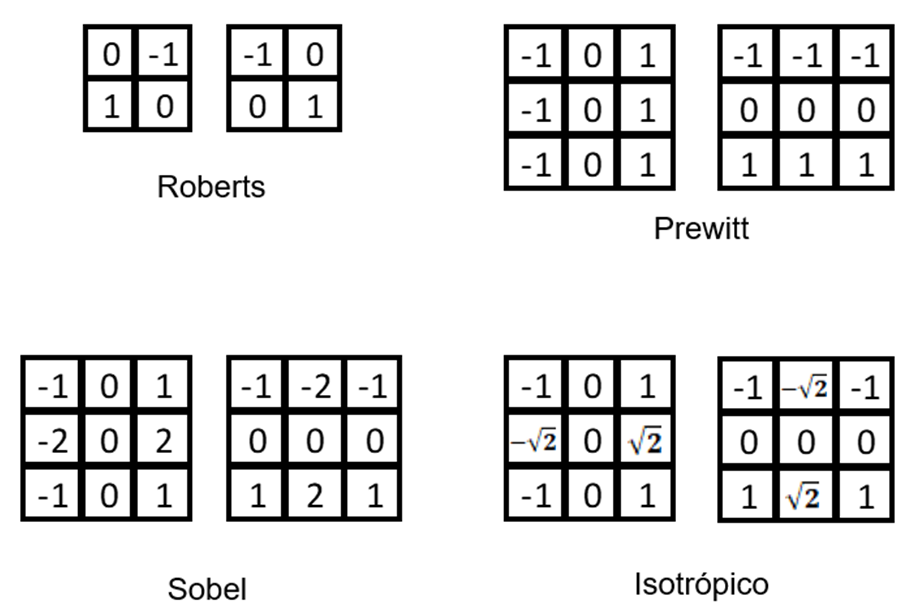
\includegraphics[scale=0.6]{Img_filtros-gradiente.png}
        \caption{Máscaras de filtro Roberts, Prewitt, Sobel e isotrópico.}\label{Fig:MFG}
    \end{figure}


\section{Estado del arte}

    \subsection{Evaluación clínica para tratamientos de cáncer de pulmón}
    En 1981, la Organización Mundial de la Salud (OMS) publicó unas directrices que proporcionan criterios estándar para evaluar la respuesta a los tratamientos contra el cáncer en ensayos clínicos. Este enfoque de referencia se concibió para investigar la importancia de los tratamientos contra el cáncer mediante una estimación del tamaño del área tumoral. Más tarde, en el año 2000, aparecieron los  criterios RECIST y su enfoque se centró en la medición del diámetro máximo. y posteriormente, los nuevos criterios que aparecieron en la literatura se basan en la versión anterior de RECIST. En resumen, estos enfoques emergentes extendieron su aplicación a ciertos tipos de tratamiento o abordaron el seguimiento de tipos particulares de cáncer. La investigación también aborda la cuestión de reconocer los beneficios y los inconvenientes de las mediciones de área y volumen en imágenes de TC. En este caso, el propósito es determinar cuándo estas mediciones se correlacionan mejor con la supervivencia del paciente. Hasta ahora, no se ha demostrado que las mediciones de área y volumen evalúen mejor la respuesta al tratamiento que la medición unidireccional en el cáncer de pulmón. La tabla \ref{tab:MEASUDIMENSIONS} reúne literatura completa sobre este eje de investigación.\\

    \begin{table}[h]
        \caption{Artículos de radiología con diferentes dimensiones de medición aplicadas a los criterios de evaluación del tratamiento.\label{tab:MEASUDIMENSIONS}}
        \begin{tabular}{p{4cm} p{2.5cm} l p{2.2cm} l}
        \hline
        \bf{Objeto principal} & \bf{Criterios} & \bf{Medición} & \bf{Tipo de cáncer} & \bf{Referencia} \\
        \hline
        Comparar diferentes enfoques de medición. & RECIST & 1D, 2D y 3D & Pulmón & \cite{WernerWasik2001} \\
        \hline
        Comparar diferentes criterios & OMS y RECIST & 1D y 2D & Gástrico, pulmón, mama e hígado& \cite{Park2003} \\
        \hline
        Comparar diferentes intervalos de corte. & OMS y RECIST 1.1 & 1D, 2D y 3D & Pulmón & \cite{Zhao2013} \\
        \hline
        Comparar enfoques de medición (esférica 3D y elipsoide vs. 1D). & RECIST 1.1 & 1D y 3D & Pulmón & \cite{Petrick2014} \\
        \hline
        Examinar las correlaciones entre las mediciones 1D y 3D. & RECIST 1.1 & 1D y 3D & Pulmón & \cite{Hayes2016} \\
        \hline
        Analizar RECIST con varios tipos de tumores y diferentes tratamientos. & RECIST 1.1 & 1D & Pulmón, mama y colon & \cite{litiere2019} \\
        \hline
        \end{tabular}
        \end{table}

        La literatura indica un acuerdo poco claro respecto al uso de la medición volumétrica para la evaluación de la respuesta tumoral. Algunos estudios anteriores como el de \cite{Hayes2016} indican que la evaluación volumétrica está más correlacionada con los resultados de supervivencia que los criterios RECIST 1.1, mientras que otros estudios no han indicado ningún beneficio particular para la evaluación volumétrica (\cite{WernerWasik2001}). Además, el uso de la evaluación volumétrica no mostró un beneficio sobre los criterios RECIST 1.1 hasta cierto punto, esto puede explicarse por el hecho de que no hay acuerdo sobre los umbrales volumétricos exactos que deberían usarse para estar perfectamente correlacionados con los umbrales unidimensionales de RECIST 1.1 y diversos autores sugieren que diferentes sitios de enfermedad pueden tener diferentes umbrales volumétricos. Los criterios RECIST han tenido un éxito notable y se han aplicado para evaluar la respuesta tumoral en miles de estudios clínicos,  pero otra forma de realizar un evaluación de respuesta a tratamientos es por medio de los cambios metabólicos en los tumores, los estudios de imagen metabólicos PET o las técnicas híbridas PET/TC, forman parte integral de la oncología actual.\\

        En oncología el radiotrazador más utilizado es la fluorodeoxiglucosa marcada con F18 (F18-FDG), que permite detectar tumores malignos, sin embargo, su dependencia de un examen morfológico complementario para una adecuada interpretación, asociado a su poca disponibilidad han obstaculizado su uso clínico masivo. El PET/TC representa una importante herramienta en el diagnóstico, estadificación y seguimiento de diversas neoplasias, particularmente del cáncer pulmonar (\cite{Guevara2010}).Cuando se discuten los criterios para la evaluación de la respuesta tumoral mediante PET con FDG y cambios en el metabolismo tumoral, es importante considerar la historia de los criterios de respuesta morfológica, que muestra que criterios simples pueden resultar muy valiosos si son sólidos y se utilizan de forma rutinaria en ensayos clínicos. Los criterios de respuesta PET de la EORTC y PERCIST siguen el modelo de RECIST y definen cuatro categorías de respuesta similares a RECIST. Sin embargo, existen algunas diferencias en las definiciones exactas de las categorías de respuesta y PERCIST proporciona muchos más detalles sobre qué lesiones se consideran mensurables y cómo se deben analizar las exploraciones con múltiples lesiones, esto a contribuido a un mayor uso de los criterios PERCIST y es probable que PERCIST reemplace los criterios de la EORTC de la misma manera que RECIST ha reemplazado los criterios de la OMS. \cite{Pinker2017} realizaron  un extenso análisis en cuanto a las diferencias entre los criterios EORTC y PERCIST, donde la principal diferencia es el uso de SUV normalizados por la masa corporal magra, no por el área de superficie corporal y un enfoque diferente para seleccionar las lesiones en la línea de base y exploración de seguimiento. \cite{Pinker2017} mencionaron que en muchos estudios se han utilizado SUV máximos o medios para cuantificar la captación de FDG tumoral, pero tienen limitaciones específicas. Los SUV máximos son muy fáciles de medir de forma independiente del operador, pero son sensibles al ruido de la imagen y pueden sobreestimar la captación tumoral de FDG en lesiones levemente ávidas de FDG, por ejemplo, metástasis después de la quimioterapia. Los SUV promedio evitan este problema, pero requieren la definición de los límites del tumor y esta definición de los bordes del tumor introduce variabilidad entre observadores, porque frecuentemente es necesario separar la captación fisiológica de FDG por captación patológica del tumor. El objetivo de SUV pico es evitar las limitaciones de SUV maximo  y SUV medio midiendo la concentración de actividad en un volumen de aproximadamente 1,0 $cm^3$ que abarcan los píxeles con la mayor concentración de radiactividad en el tumor. Finalmente sus estudios han demostrado que los criterios de la EORTC y PERCIST proporcionan una evaluación muy similar de la respuesta tumoral, sin embargo, determina que PERCIST ha perfeccionado la evaluación y proporciona un marco mucho más detallado para la selección de lesiones, la definición de la región de interés y la clasificación de la respuesta.\\
 
    \subsection{Aplicación de radiomica en cáncer de pulmón}
    En los últimos años, el aprendizaje profundo, ha emergido como una herramienta poderosa para el procesamiento de imágenes, debido a que puede analizar grandes cantidades de datos, en imágenes médicas utilizando CNN, o procesando datos genómicos e información clínica, para identificar patrones y hacer predicciones con el uso de RNN. \cite{Trebeschi2019} y \cite{Chen2020} trabajaron con modelos CNN para la predicción de la respuesta a la lesión pulmonar basándose en características extraídas de TC, \cite{Chen2020} utilizaron las características extraídas para la clasificación de las lesiones pulmonares realizando una segmentación automática para extraer sus volúmenes 3D y \cite{Trebeschi2019} se centraron en un método que  refleja la condición metastásica que caracteriza a los pacientes que reciben inmunoterapia. Otro enfoque de relacionado a la extracción de características fue \cite{Chaunzwa2021} que utilizaron las CNN para predecir la histología tumoral del CPCNP con un enfoque en los dos tipos histológicos más comunes: adenocarcinoma y carcinoma de células escamosas, este enfoque podría servir como ayuda correctiva para los diagnosticadores y clasificadores de tipos de cáncer. Por su parte \cite{Deng2023} desarrollaron su modelo de aprendizaje profundo para diferenciar pacientes con cáncer de pulmón en etapa cuatro mediante imágenes TC previas a la terapia y predecir los beneficios de supervivencia a la terapia EGFR-TKI e ICI. \cite{Gainey2023} desarrollaron un modelo de aprendizaje profundo para el pronóstico supervivencia libre de progresión local, supervivencia general y  la supervivencia específica de la enfermedad, basado en segmentación de imágenes TC en pacientes con cáncer de pulmón de células no pequeñas tratados con radioterapia corporal estereotáxica, donde se concluyo que El modelo propuesto tiene el potencial de ser un complemento a los criterios RECIST 1.1.\\
    
        \subsubsection{Clasificación para diagnostico}
        Otra forma de utilizar las características extraídas de imágenes TC es para propósitos de diagnostico del cáncer, en ese sentido \cite{Gopinath2023}, \cite{Raza2023}, \cite{Rajasekar2023}, \cite{Maleki2023} y \cite{Wankhade2023} trabajaron con arquitecturas CNN y RNN para determinar si un tumor es benigno o maligno. Una fase recurrente en estas investigaciones es la aplicación de técnicas de preprocesamiento en las imágenes, \cite{Gopinath2023} exploraron la aplicación de eliminación de ruido para mejorar los resultados de diagnóstico, \cite{Raza2023} utilizaron el redimencionamiento para eliminar regiones no deseadas como fondo y ruido que podrían causar un entrenamiento ruidoso y de esta forma mejorar los resultados en la clasificación. \cite{Maleki2023} por su parte, además de utilizar la eliminación de ruido y redimensionamiento en el preprocesamiento también añadieron la segmentación previa para delimitar el área y eliminar zonas innecesarias de la imagen, como conclusión su modelo de clasificación mejora significativamente al añadir 6 técnicas de extracción de características (Filtro Gabor, filtro sobel, filtro Schar, Filtro Prewitt, Filtro Guassiano y Roberts). Finalmente \cite{Wankhade2023} utilizaron la conversión a escala de grises, la reducción de ruido, la segmentación y normalización como técnicas de preprocesamiento para su técnica híbrida CNN y RNN que fue capaz de realizar un buen diagnóstico en etapas tempranas del cáncer pulmonar.\\
        
        \subsubsection{Metodologías usadas en la evaluación de tratamientos}\label{sec:3.2.2}

        Los esfuerzos orientados a la investigación en sistemas de atención médica inspirados en el aprendizaje automático están diseñados para ayudar a los procedimientos clínicos a los que deben someterse los pacientes con cáncer de pulmón. La mayoría de los avances actuales en este campo tratan del diagnóstico de enfermedades realizado mediante modelos CNN de clasificación. Sin embargo, el campo DL ha desempeñado un papel en la realización de otros procedimientos médicos. Una razón para ampliar el alcance de la aplicación del DL durante los procedimientos de seguimiento de los pacientes con cáncer de pulmón es que su pronóstico suele ser adverso porque, muchas veces, la enfermedad se detecta tarde. Una medida que podría aliviar este pronóstico sería reconocer tratamientos eficaces para cada paciente. Los tratamientos contra el cáncer comprenden cirugía, radiación, medicamentos y otras terapias para curar el cáncer, reducir el tamaño de los tumores o detener la progresión del cáncer. El presente estudio profundiza en las técnicas de aprendizaje automático que pueden formar parte de nuevos sistemas inteligentes concebidos para ayudar al seguimiento de los tratamientos del CPCNP o de los ensayos clínicos basados en imágenes de TC y PET.\\

        Los cambios morfológicos encontrados en las lesiones cancerosas son la medida estándar para evaluar los tratamientos contra el cáncer. Como se señaló en la Sección~\ref{seccion:CBMC}, clínicamente, RECIST proporciona las pautas que estandarizan los criterios para medir cómo responde un paciente con cáncer al tratamiento. El monitoreo de la enfermedad asistido con métodos de DL a menudo utiliza RECIST para entrenar los algoritmos o modelos formados por arquitecturas de redes neuronales profundas. La Fig.~\ref{fig:SSE} en la Sección~\ref{Section:TEM} describe las principales etapas de un método de DL para el monitoreo del tratamiento del cáncer. Un desafío significativo es automatizar todo el proceso por completo. Los métodos de DL suelen implicar entradas manuales. Algunas publicaciones de investigación abordan procedimientos de notación, segmentación o clasificación de respuestas automatizados o semiautomatizados. \\

        \cite{Chang2022}, por ejemplo, desarrolló un método basado en DL para predecir la respuesta al tratamiento de pacientes con CPCNP sometidos a quimioterapia. El método utiliza imágenes de TC como entrada. Se entrena una red neuronal profunda para clasificar la respuesta del tumor a la quimioterapia. El resultado es el pronóstico entre \textit{respuesta} (que se refiere a CR y PR) y \textit{sin respuesta} (para PD y SD). El método de evaluación del tratamiento del cáncer diseñado por IA aprovecha las herramientas de DL habituales en el procesamiento de imágenes de conjuntos de datos de dos hospitales. La red troncal se entrenó previamente con imágenes de la base de datos ImageNet. La eficacia en la predicción de la evolución del tumor mediante el método DL se evaluó comparando su resultado con la decisión de los radiólogos que aplicaron las pautas RECIST. El enfoque propuesto tiene tres características: se basa en el modelo de aprendizaje de instancias múltiples (MIL). El problema MIL, que se describe más adelante, es una clase de aprendizaje supervisado en la que se asignan múltiples instancias observadas a una sola etiqueta de clase (\cite{Javed2022}). Se probaron varias CNN de la red troncal entrenadas previamente como redes de extracción de características. Estas redes trataron los datos de entrada en una representación de características específica. \\

        El enfoque descrito utilizó el etiquetado de una serie de imágenes en lugar de cada corte. En los problemas de clasificación de imágenes habituales, el aprendizaje supervisado estándar entrena modelos predictivos mediante el mapeo entre instancias de entrada o vectores de características y salidas o etiquetas. En tales casos, el conjunto de datos de entrenamiento incluye pares de entrada-salida, con instancias etiquetadas con una clase específica. Otro escenario ocurre cuando hay múltiples instancias presentes con una declaración de clase general. Este escenario ocurre, por ejemplo, en imágenes de cáncer de pulmón, donde la etiqueta de benigno o maligno puede describir la imagen, o se proporciona de manera rudimentaria una Región de interés (ROI). El llamado enfoque de aprendizaje de instancias múltiples (MIL) está programado en ese caso. Es el método de aprendizaje utilizado para datos con anotaciones débiles. Las etiquetas de clase MIL se definen y asignan globalmente a imágenes o bolsas. Luego, el sistema aprende a detectar patrones relevantes en estas imágenes localmente. MIL supera las limitaciones del aprendizaje supervisado estándar cuando las etiquetas de instancias individuales no están disponibles. En \cite{waqas_exploring_2024,ilse18a,quellec_multiple-instance_2017} se ofrece una serie de trabajos de investigación que explican el enfoque MIL profundo. \cite{ilse18a} informó diferentes métodos para resolver la tarea de clasificación. \\

        Muchas investigaciones abordan cuestiones prácticas para mejorar el rendimiento de las redes neuronales o probar las herramientas de DL. En este contexto, \cite{holliday_pre-trained_2020} proporcionó un análisis particular que ayuda a evaluar el rendimiento de las CNN preentrenadas como extractores de características en aplicaciones de coincidencia visual. El estudio abarcó varias arquitecturas de CNN de diferentes familias, como AlexNets, VGG Nets, ResNets y DenseNets. Cabe señalar que \cite{Chang2022} probó todas estas familias de CNN. El análisis brindó información para evaluar la solidez de las características de las CNN ante cambios de apariencia, escala y perspectiva. Estos análisis de la robustez de CNN se pueden extender a diferentes arquitecturas y pueden ayudar a elegir una arquitectura específica. \\

        Como se ha mencionado RECIST se basa en la medición 1D de las lesiones para evaluar la respuesta terapéutica en tumores sólidos. En este contexto, \cite{Arbour2021} presentó un enfoque centrado en el desarrollo de un modelo DL para estimar la mejor supervivencia general y la supervivencia de la enfermedad no evolutiva después del tratamiento específico del cáncer de pulmón. Este proyecto tuvo como objetivo promover la evaluación de grandes bases de datos clínicas de la cantidad significativa de pacientes tratados fuera de los ensayos clínicos. Después de eso, el objetivo fue delinear un enfoque general de evaluación del tratamiento. La idea era utilizar datos recuperados de registros médicos y no directamente de exploraciones. En cualquier caso, los datos de texto se adquirieron de las exploraciones. El modelo DL se construyó con una arquitectura de red profunda para estimar la respuesta RECIST utilizando, como entrada, texto de informes de radiología clínica de pacientes con CPCNP avanzado tratados con bloqueo de PD-1/PD-L1. La red neuronal profunda se construyó con codificación, interacción y dos capas completamente conectadas con una función de activación tangente hiperbólica. Una capa de salida con una función de activación softmax sigue a las capas anteriores. El modelo fue entrenado con informes RECIST de referencia obtenidos por radiólogos calificados. La respuesta predicha por el modelo mostró una alta similitud con la categorización RECIST. Un hallazgo del estudio es la confianza generada en los criterios RECIST estandarizados para la evaluación del tratamiento oncológico. Esto resulta de la afirmación de que el desempeño del método basado en DL fue consistente independientemente del estilo de informe del radiólogo de las instituciones seguidas. Sin embargo, se necesitan más estudios para establecer la aplicabilidad y generalización del método a otros regímenes de tratamiento. \\

        Enmarcado en el conocimiento de los cambios morfológicos, un camino sistemático hacia sistemas de monitoreo inteligente implica tareas como detección de lesiones, segmentación y medición en imágenes escaneadas. Luego, los datos obtenidos se guían hacia funciones de comparación y evaluación. Varias técnicas de IA para el pretratamiento y filtrado pueden mejorar el procesamiento de imágenes. Los pasos críticos en el manejo de imágenes son la segmentación y la creación de marcadores en imágenes preseleccionadas con CNN. El conjunto de herramientas de DL tiene como objetivo facilitar el procedimiento de medición de imágenes de TC para radiólogos. En algunos desarrollos, el procedimiento está automatizado hasta cierto punto. El procesamiento de imágenes automatizado o autoconfigurable compensa las mediciones inconsistentes y sesgadas entre los radiólogos. Por ejemplo, \cite{Tang2018} creó un método unidimensional (1D) semiautomático que utiliza una CNN en cascada para etiquetar el procedimiento RECIST. El método comienza definiendo la región de interés (ROI), que un radiólogo dibuja manualmente utilizando un cuadro marcado para limitar el área seleccionada. Se construyó una CNN con dos redes neuronales profundas en cascada. La primera es una red de transformadores espaciales (STN) con tres partes: una red de localización, un generador de cuadrícula y un muestreador. Esta STN predice transformaciones de traslación, rotación y escalado de la lesión en función de una matriz de transformación. Se creó para controlar la normalización de la región de la lesión, por medio de la cual el método general se vuelve robusto a la variabilidad en tamaños, ubicaciones y orientaciones en diferentes imágenes. Se utiliza una red de reloj de arena apilada SHN en la cascada para la estimación RECIST. Después de la transformación de la imagen, SHN estima las posiciones de los puntos finales de tal manera que se aproxima a los diámetros más largo y más corto de la lesión. La estructura de SHN involucró capas convolucionales, de agrupamiento máximo y de sobremuestreo que brindan precisión a la predicción RECIST. \\

        \cite{Xie2021} analizó los desafíos y los diversos enfoques para la detección de lesiones. Esta investigación se centró en el desarrollo de un método de anotación para imágenes de lesiones de cáncer de pulmón. Su método, RECIST-Net, fue diseñado como una nueva CNN con un enfoque para detectar cuatro puntos extremos y el punto central de la lesión. \\

        La segmentación de las lesiones y su posterior conversión a una medición unidireccional según la guía RECIST son pasos fundamentales en la automatización del procesamiento de imágenes. La medición automatizada es un desafío cuando los marcadores visuales de los puntos finales y las áreas circundantes de una lesión son difíciles de discernir. También es un desafío cuando se necesita una interpretación clínica significativa o la elucidación de la lesión. Por el contrario, la segmentación de la lesión y la conversión de la medición se pueden automatizar fácilmente si los límites de la lesión están bien definidos. Estos aspectos fueron analizados por \cite{Woo2021}, quien también contribuyó con un método semiautomático para mediciones 1D en imágenes de TC utilizando CNN. El método involucró tres CNN en cascada entrenadas para etiquetar si el tamaño de una lesión objetivo es mayor o menor a 32 píxeles. El conjunto de CNN DL no logró clasificar cuando el tamaño de la lesión coincidía con 32 píxeles. Los pasos de pretratamiento de la imagen fueron los siguientes: primero, se redimensionaron las imágenes de TC. Las mediciones 1D pasaron de centímetros a píxeles. Luego, las imágenes se ampliaron mediante interpolación bicúbica. Las lesiones objetivo se colocaron en un marco de 128 x 128 píxeles con el punto de medición central como centro del marco. El método utiliza un punto arbitrario dentro de la lesión objetivo como entrada. Por esta razón, no es un algoritmo completamente automatizado. Sin embargo, el método propuesto mostró una excelente concordancia con las mediciones realizadas por un radiólogo. Este trabajo es una base para integrar aún más modelos para detectar una lesión, identificar un punto arbitrario dentro de la lesión y tomar mediciones utilizando el punto de entrada para automatizar el proceso. \\

        También se han desarrollado métodos DL para la segmentación volumétrica de imágenes de TC de lesiones de cáncer de pulmón. \cite{Jiang2019} trabajó con un enfoque de CNN de múltiples escalas para segmentar volumétricamente tumores y nódulos de CPCNP de pacientes sometidos a inmunoterapia, que altera el tamaño y la apariencia de los tumores. Este trabajo abordó la variabilidad de la segmentación semiautomática encontrada en varios métodos informados en la literatura. En la misma línea de la segmentación de imágenes de TC, \cite{Chen2021} desarrolló una nueva arquitectura de CNN basada en codificador-decodificador para segmentar lesiones tumorales con precisión. \cite{Kidd2022} propuso un método que profundizó más en la automatización de la medición de lesiones cancerosas. Avanzó hacia la medición del volumen del mesotelioma pleural maligno (MPM), una forma rara y grave de cáncer que se origina en la membrana que recubre los pulmones y el interior de las costillas. Lo más destacado de esta estrategia es su carácter de automatización completa para evaluar la respuesta de la quimioterapia al MPM. Como tal, el enfoque de segmentación basado en CNN no requiere ninguna entrada manual. Las anotaciones manuales de especialistas solo se utilizaron como un medio para entrenar la segmentación y validar la volumetría del MPM. Este método utilizó una CNN con arquitectura bidimensional para segmentar cada intervalo de corte axial de la TC. Clasificó la respuesta y evaluó el rendimiento del método basado en DL con criterios mRECIST. Como resultado, el resultado del método cumplió con la evaluación de los especialistas en un grado aceptable. Sin embargo, el método se considera una prueba de principio que respalda la viabilidad de herramientas similares y más precisas. En la misma línea, otros trabajos que abordan la segmentación automatizada de imágenes de cáncer de pulmón se reúnen en la Tabla~\ref{tab:SegRef} con sus métricas de evaluación informadas mencionadas en la sección~\ref{sec:2.5.6}. Para los trabajos de investigación citados, la información proporcionada incluye la clase de red neuronal profunda utilizada, el enfoque dimensional para la medición de la lesión y la puntuación de evaluación. En la Tabla~\ref{tab:TCDatabase} del Anexo B, se muestran las bases de datos utilizadas para el entrenamiento.

        \begin{table}[H]
            \caption{Artículos basados en la segmentación del cáncer de pulmón en imágenes de TC.\label{tab:SegRef}}
            \begin{center}
            \begin{tabular}{p{2.8cm} p{4cm} p{3.2cm} p{3.5cm}}
            \hline
            \textbf{Referencia} & \textbf{Método} & \textbf{Enfoque dimensional} & \textbf{Puntaje de evaluación} \\ \hline
            \cite{Alakwaa2017} & CNN (U-Net) & 3D & 86.6\% (ACC) \\
            \hline
            \cite{Liu2018} & Mask R-CNN & 2D & 79.65\%(ACC) \\
            \hline
            \cite{Jiang2019} & CNN (U-Net) & 2D & 72\%(ACC), 75\%(DC), 82\%(SEN) \\
            \hline
            \cite{Baek2019} & CNN (U-Net) & 3D & 82,8\%(DC) \\
            \hline
            \cite{Hu2020} & Mask R-CNN & 2D & 89.96\%(ACC), 76.81\%(DC), 87.72\%(SEN), 86.7\%(SPE) \\
            \hline
            \cite{Yang2021} & CNN (MSDS-UNet) & 3D & 69.1\%(DC), 74.4\%(SEN) \\
            \hline
            \cite{Tan2021} & GAN & 2D & 98.5\%(ACC) \\
            \hline
            \cite{Gainey2021} & CNN (U-net) & 3D & 78\%(DC) \\
            \hline
            \cite{Dutande2021} & CNN (SquExUNet) & 3D & 80\%(DC) \\
            \hline
            \cite{Chen2021-2} & CNN (SegNet) & 2D & 92.5\%(ACC), 95.11\%(DC), 98.33\%(SEN), 86.67\%(SPE) \\
            \hline
            \cite{Salama2021} & CNN (ResNet50,U-Net) & 2D & 98.43\%(ACC), 98.86\%(DC), 98.99\%(SEN) \\
            \hline
            \cite{Primakov2022} & CNN (U-Net) & 3D & 82\%(DC) \\
            \hline
            \cite{Aversano2022}& CNN (GUNET3++) & 2D & 96\%(DC) \\
            \hline
            \cite{Cifci2022} & CNN (SegChaNet) & 3D & 98.48\%(DC) \\
            \hline
            \cite{Le2023} & CNN (RRc-Unet) & 3D & 87.77\%(DC) \\
            \hline
            \cite{V2023} & CNN (Unet) & 2D & 82\%(ACC), 62\%(DC) \\
            \hline
            \cite{Wu2023} & CNN (RAD-UNet) & 2D & 88.13\%(DC), 92.17\%(SEN), 94.75\%(SPE) \\
            \hline
            \cite{kunkyab2024} & CNN, Transformer & 2D & 92\%(DC) \\
            \hline
            \end{tabular}
            \end{center}
            \begin{tabular}{l}
            \footnotesize ACC: Precisión \\
            \footnotesize DC: Coeficiente Dice \\
            \footnotesize SEN: Sensibilidad \\
            \footnotesize SPE: Especificidad \\
            \end{tabular}
        \end{table}




        La tomografía por emisión de positrones (PET) es una de las técnicas de diagnóstico por imágenes estándar para el cáncer de pulmón y la evaluación de tratamientos liderados por médicos oncólogos que intentan encontrar una cura para esta enfermedad. La tomografía por emisión de positrones utiliza fluorodesoxiglucosa (FDG) para caracterizar la lesión en un marco de referencia fisiológico y metabólico. Este medio permite exponer la textura heterogénea y los contornos variables de los nódulos. La información así obtenida puede no revelarse en las imágenes de TC \cite{Chen2022,Coleman1999,Coleman2006}. Por otro lado, las exploraciones metabólicas y anatómicas pueden proporcionar información complementaria. Al igual que las pruebas basadas en TC, la evaluación metabólica por PET es un método sistemático que necesita un alto grado de experiencia con criterios consistentes para funcionar bien. Por su naturaleza, la técnica PET es pronóstica. La evaluación de la respuesta al tratamiento de los cánceres sólidos mediante cambios metabólicos es más eficaz y rápida que las evaluaciones anatómicas. Sin embargo, las diversas condiciones para su uso y la baja disponibilidad de equipos para realizar esta prueba en los centros oncológicos conducen a un uso menos frecuente de la PET en la evaluación clínica. En la literatura se proponen métodos de aprendizaje profundo que utilizan imágenes PET o exploraciones PET/CT combinadas como entrada para los algoritmos diseñados para aprendizaje profundo \cite{Weyts2024}. \\

        Los siguientes estudios en el campo se describen para identificar las herramientas y objetos de aprendizaje profundo utilizados, los pasos de procesamiento de imágenes para tratar las imágenes PET y las diversas tareas involucradas en los diseños de métodos de aprendizaje profundo que son prácticos para la detección del cáncer de pulmón y el seguimiento del tratamiento, con un enfoque particular en el segundo objetivo. \\

        Recientemente se han desarrollado varios métodos de aprendizaje profundo para la detección de CPCNP. \cite{Zhang2019} presentó un método CNN basado en regiones de múltiples escalas que utiliza imágenes PET para detectar candidatos a tumores pulmonares. Esta estrategia utiliza tres modelos de Mask R-CNN, cuyas funciones son la detección y segmentación de objetos. Los modelos se ajustaron y entrenaron con conjuntos de datos utilizando tres escalas diferentes. Luego, se implementó un enfoque de votación ponderada o toma de decisiones para disminuir los resultados falsos positivos. El Max R-CNN aplicado es una extensión del R-CNN o CNN basado en regiones, un algoritmo de detección de objetos simple y escalable. Un algoritmo intermedio mejorado, Faster R-CNN, logra flexibilidad y robustez. Clasifica los objetos pero no encuentra qué píxel es parte de un objeto en una imagen. Mask R-CNN mejora el Faster R-CNN insertando una función para predecir máscaras de segmentación en los RoI junto con los elementos de regresión de cuadro delimitador y clasificación actuales \cite{He2017}. Sus funciones son detección de objetos y segmentación semántica. Del mismo modo, para la detección de NSCLC, \cite{Chen2022} presentó un método CNN 3D guiado por atención multimodal para la detección de NSCLC en imágenes PET/CT combinadas. Los mecanismos de atención son una clase de capas de red neuronal que permiten que el modelo enfatice partes específicas de la entrada ponderando la entrada de acuerdo con la relevancia de las entradas con respecto a la tarea en cuestión. Como resultado, este trabajo registró una ventaja en la detección de casos que podrían pasar desapercibidos mediante la evaluación visual. \\

        Algunos trabajos van más allá en la evaluación asistida por IA de los cambios metabólicos. La segmentación en imágenes PET de la captación de FDG es fundamental para realizar una evaluación precisa del tumor. El estudio dirigido por \cite{Fruh2021} tuvo como objetivo desarrollar un método DL para la segmentación débilmente supervisada de lesiones tumorales a partir de imágenes PET/CT preprocesadas. Este enfoque reduce la complejidad de la etiqueta y, por lo tanto, disminuye la acción humana en el entrenamiento del modelo. La máscara de segmentación se diseñó de la siguiente manera. Un radiólogo, corte por corte, anotó manualmente las lesiones. Con las etiquetas "tumor" y "no tumor", se entrenó una CNN con arquitectura base VGG-16 para la clasificación. El modelo VGG-16 es una CNN con una profundidad de 16 capas, 13 capas convolucionales y tres capas completamente conectadas. Esta arquitectura es simple y eficiente para tareas de visión artificial, como la clasificación de imágenes y el reconocimiento de objetos. El algoritmo propuesto diferencia cortes con y sin lesiones tumorales ávidas por FDG. Posteriormente, se generaron mapas de activación de clase (CAM) o mapas de prominencia utilizando varios métodos (CAM, GradCAM, GradCAM++ y ScoreCAM) para identificar las regiones tumorales relevantes para la decisión de la red. Se logró una segmentación de imágenes adaptativa en la región propuesta por el algoritmo CAM. Las métricas de puntuación de Dice 3D, volumen tumoral metabólico (MTV) y glicólisis total de la lesión (TLG) estimaron su rendimiento. \\

        El desarrollo de métodos de DL se enfrenta a la necesidad de manejar una gran cantidad de imágenes. Para superar este problema, \cite{Protonotarios2022} presentó un método de DL con un esquema de aprendizaje de pocos disparos basado en una arquitectura U-Net ampliamente utilizada. La conveniencia de este enfoque proviene del hecho de que el modelo utiliza menos datos para el entrenamiento. Su estrategia se vuelve adecuada al incorporar la retroalimentación del usuario para mejorar constantemente la precisión en la segmentación de lesiones de cáncer de pulmón de exploraciones PET/CT.Se remite al lector a diversos trabajos que desarrollan aún más los métodos de DL basados en U-NET o V-NET modificados como clases de CCN para la segmentación de imágenes. Estos estudios se agrupan en la Tabla~\ref{tab:petSegRef} con sus métricas de evaluación informadas mencionadas en la sección~\ref{sec:2.5.6}. En la Tabla~\ref{tab:PETDatabase} del Anexo B, se muestran las bases de datos utilizadas para el entrenamiento. Las CNN utilizadas con arquitectura modificada logran una segmentación más precisa y automatizada del ROI en imágenes FDG-PET.\\

        \begin{table}[H]
            \caption{Artículos basados en la segmentación de ROI en imágenes PET.\label{tab:petSegRef}}
            \begin{center}
            \begin{tabular}{p{3.5cm} p{4cm} p{2.3cm} p{3cm}}
            \hline
            \bf{Referencia} & \bf{Método} & \bf{Enfoque dimensional} & \bf{Evaluación}\\ 
            \hline
            \cite{Theophraste2018} & CNN (U-Net) & 3D & 93\%(DC) \\
            \hline
            \cite{Zhao2018} & CNN (V-Net) & 3D & 83\%(DC) \\
            \hline
            \cite{Leung2020} & CNN (mU-Net) & 3D & 87\%(DC) \\
            \hline
            \cite{Park2022} & CNN (U-Net) & 3D & 78\%(DC) \\
            \hline
            \cite{Lei2022} & CNN (R-CNN) & 2D & 84\%(DC) \\
            \hline
            \cite{Xia2023} & CNN & 2D & 86\%(DC), 83\%(SEN) \\
            \hline
            \cite{Yu2023} & CNN (U-Net) & 3D & 84,4\%(DC), 83\%(SEN), 84\%(SPE) \\
            \hline
            \end{tabular}
            \end{center}
            \begin{tabular}{l}
            \footnotesize DC: Coeficiente de Dice \\
            \footnotesize SEN: Sensibilidad \\
            \footnotesize SPE: Especificidad \\
            \end{tabular}
        \end{table}

        La evaluación clínica de los tratamientos del cáncer de pulmón consiste en comparar las mediciones previas y posteriores al tratamiento para determinar la respuesta según los criterios especificados en la Tabla~\ref{tab:SUVRESPONSES}, Sección \ref{seccion:CBMC}. Hasta donde sabemos, la investigación actual sobre el tema no aborda la automatización completa de estas mediciones. La literatura que aborda los métodos de DL que se basan en el procesamiento de imágenes PET presenta varios enfoques para clasificar una predicción positiva o negativa de los tratamientos contra el cáncer que operan con características radiómicas extraídas por CNN. En este sentido, \cite{Amyar2022} propuso un marco de DL de múltiples escalas para predecir la supervivencia y la respuesta al tratamiento de pacientes con cáncer de esófago y pulmón. Su método tiene como objetivo entrenar una red neuronal, clasificar la patología, segmentar la lesión, reconstruir la imagen y predecir los resultados de la segmentación. Se eligió la U-Net como la columna vertebral para procesar imágenes médicas en 3D. La idea principal era extraer información de las regiones intratumorales y peritumorales para mejorar las evaluaciones radiómicas clásicas. Su estrategia fue proponer una red de aprendizaje multitarea para alimentar características globales a la CNN con el fin de lograr la segmentación del tumor en exploraciones PET 3D mientras se impulsan las tareas de clasificación y reconstrucción. La arquitectura comprendía partes de codificación y decodificación (estas últimas para la reconstrucción y la segmentación) y conexiones de salto entre ellas. Se utilizó un perceptrón multicapa (MLP) para clasificar una CNN para la predicción de resultados después del resultado de la segmentación. \\

        \cite{Li2024} propuso otra estrategia al desarrollar un modelo DL capaz de predecir con precisión la expresión de PD-L1 (proteína de muerte celular programada-1) en pacientes con CPCNP sometidos a inmunoterapia basándose en datos de TC/TEP. Este método proporciona una herramienta no invasiva para que los médicos seleccionen pacientes con PD-L1 positivo. Los especialistas describieron la región de interés (ROI, por sus siglas en inglés). Esta ROI, junto con las imágenes originales de TC y TEP, se introdujeron en el módulo PyRadiomic para extraer características radiómicas. Este paquete de código abierto está programado en Python para extraer características radiómicas de imágenes médicas. En el trabajo citado, se extrajeron características adicionales mediante análisis de imágenes de alta dimensión con filtros de imagen, como filtros Wavelet y Gaussianos. Se utilizó una CNN con arquitectura ResNet-101 para la extracción de características de las imágenes TEP/CT. La ResNet-101 es una CNN que tiene 101 capas de profundidad y existe una versión preentrenada en la base de datos ImageNet. Un radiólogo seleccionó una región delimitadora rectangular que encierra el tumor. La información se manipuló para ingresar al software de extracción de características. Un análisis de regresión logística favoreció la combinación de radiómica y firmas de aprendizaje profundo para calcular la probabilidad total de PD-L1 positivo. Al final, los métodos estadísticos ayudaron a diferenciar las características clínicas en pacientes con CPNM con PD-L1 positivo y negativo. Además, se evaluó estadísticamente el rendimiento del modelo para determinar su precisión, sensibilidad y especificidad.\\

        Se informó que se utilizaron algunas bases de datos de entrenamiento en la investigación citada para recopilar imágenes TEP. La Tabla~\ref{tab:PETDatabase} anexo D, muestra algunas de estas bases de datos disponibles.\\

        En cuanto a la medición en TEP, las técnicas de pretratamiento pueden mejorar la calidad de las imágenes. A su vez, algunos procesos, como los métodos de eliminación de ruido con IA, pueden modificar ligeramente la información de la imagen de una manera desconocida \cite{Jaudet2021}. Algunos estudios han verificado la influencia de los métodos de eliminación de ruido, que incluyen los trabajos de \cite{weyts_2022} y \cite{Jaudet2021}. Otro caso de ello es el estudio de \cite{Weyts2024}. En este estudio, se intentó avanzar para comprobar si la eliminación de ruido con IA para imágenes PET también tiene al menos un ligero impacto en la cuantificación de lesiones para la evaluación del tratamiento del cáncer según las directrices EORTC y PERCIST, ya que se ha reconocido que estos criterios estándar conducen a clasificaciones muy similares. El estudio concluyó que es factible incluir imágenes PET con eliminación de ruido con IA, y que la respuesta al tratamiento determinada clínicamente es satisfactoria para los criterios estándar clínicos EORTC y PERCIST.


    \subsection{Conclusiones}
    La información recopilada en esta sección brinda información tanto de las bases de datos de imágenes como de las métricas para evaluar el rendimiento de los métodos propuestos. Diversas métricas pueden evaluar el rendimiento, pero la calificación a menudo se basa en el \%  de precisión y el coeficiente Dice. Por lo tanto, la integración de DL en la práctica clínica necesita un proceso sistemático.\\

    La segmentación es un paso crucial en los métodos de DL. Los hallazgos de la mayoría de los estudios revisados revelan que las técnicas de DL logran una alta precisión para este propósito. Una de las fortalezas de estas técnicas es su tiempo relativamente corto para procesar los datos. Sin embargo, el entrenamiento del modelo requiere mucho tiempo y computación. La tarea de segmentación de lesiones a menudo se realiza accediendo a extensas bases de datos etiquetadas. La clasificación de CPCNP con fines de diagnóstico han logrado una buena precisión en la identificación de lesiones en imágenes clínicas. Estos enfoques enfatizan el uso de filtros para mejorar la detección de enfermedades. En contraste, estos filtros rara vez se aplican en el trabajo centrado en la segmentación. \\

    Se ha afirmado que la encuesta se enmarca en los métodos de DL desarrollados para monitorear los tratamientos de CPCNP, a partir de TC y TEP. Las lesiones en las imágenes de TC se miden actualmente utilizando diferentes enfoques que involucran mediciones de lesiones 1D, 2D y 3D. Las mediciones unidimensionales en imágenes de TC cumplen con las pautas y procedimientos RECIST. Sin embargo, numerosas investigaciones se refieren a los métodos de DL con evaluaciones de superficie y volumétricas en imágenes de TC. La medición en las tomografías por emisión de positrones es consistentemente volumétrica. Esta revisión distingue entre estos enfoques, examina sus desafíos y resultados, y presenta varios recursos computacionales y tipos de arquitecturas de redes neuronales aplicadas para desarrollar métodos de monitoreo asistido por DL utilizando tomografías computarizadas y tomografías por emisión de positrones. También se analiza el grado de automatización del método. A menudo, las entradas a los métodos de DL son anotaciones manuales y selección de ROI, lo que conduce a estrategias semiautomáticas. \cite{Liu2022} propuso una referencia de trabajo con un sistema altamente automatizado para el seguimiento del cáncer, quien desarrolló la medición 1D a partir de exploraciones de resonancia magnética y un algoritmo para segmentar las metástasis hepáticas siguiendo los criterios RECIST 1.1 y basado en CNN U-net entrenado para la segmentación. La anotación del hígado y las metástasis hepáticas se realizó mediante una plataforma de software de código abierto (ITK-SNAP). El algoritmo DL calculó el tamaño del tumor y un programa basado en reglas evaluó la respuesta al tratamiento de acuerdo con los criterios RECIST 1.1. Las tareas propuestas en este trabajo descrito son factibles de adoptar para estudiar y mejorar la práctica médica en la detección y cura del CPCNP.

    Esta revisión de la literatura se centra en los avances y herramientas potenciadas por las técnicas de Deep Learning (DL) para su aplicación en el seguimiento del tratamiento del CPCNP y en los esfuerzos por lograr métodos automatizados. Los principales avances en el tema se encuentran en los métodos de segmentación, ya que es una etapa fundamental en la automatización de los procesos clínicos basados en DL. Las arquitecturas de redes neuronales de DL pueden realizar este trabajo más rápido que un especialista tanto para pruebas morfológicas como metabólicas. Una etapa desafiante es el entrenamiento del modelo, ya que su efectividad y el consumo de tiempo son cuestiones a abordar. Otro enfoque más considerado es la predicción de la respuesta a partir de las características radiómicas extraídas de las imágenes. Esta predicción difiere de los pasos de clasificación clásicos, que son estrictos según los estándares de referencia para los métodos de evaluación del tratamiento. Por otro lado, la medición bidimensional en imágenes de TC, como etapa previa a la segmentación por redes neuronales, todavía se logra manualmente. En los métodos basados en PET, el análisis se realiza regularmente mediante medidas volumétricas. Hasta la fecha, no se han reportado métodos de DL para evaluar el tratamiento del CPCNP basado en evaluaciones clínicas metabólicas completamente automatizadas.\\

    Según los hallazgos, los tipos regularizados de redes neuronales profundas implementados para ayudar a la detección del cáncer y el monitoreo del tratamiento, tienen una base en estructuras CNN, RNN y GAN, incluidos los métodos híbridos que combinan diferentes estructuras. Para la segmentación, la estructura de red neuronal predominante es U-Net. Además, muchos trabajos han mejorado el rendimiento de los modelos de DL modificando ligeramente las estructuras nombradas. Finalmente, también hemos identificado la posibilidad de agregar herramientas de IA de preprocesamiento a las imágenes clínicas, ya que solo unos pocos trabajos revisados sobre el tema del control del tratamiento del cáncer utilizan técnicas de filtrado de imágenes. Sin embargo, los estudios centrados en el diagnóstico concluyeron que ciertos filtros han mejorado la precisión de los modelos. Además, se ha demostrado que la eliminación de ruido de IA modifica la información de la imagen, pero el efecto de estos cambios no afecta la efectividad de la evaluación del tratamiento. La investigación revisada también considera cuestiones sobre la introducción de la solidez de las características de la red neuronal y la ponderación adaptativa de parámetros en línea para mejorar la precisión de los modelos de red neuronal.
        


\section{Propuesta}

    \subsection{Planteamiento del problema}
    La evaluación clínica de tratamientos contra el cáncer de pulmon mediante imágenes supone un reto para los especialistas. Dado el nivel de experiencia y el tiempo necesario para analizar una gran cantidad de imágenes médicas, se convierte en una tarea ardua. Se puede prever que las herramientas de DL participen en el seguimiento de la respuesta del paciente al tratamiento del cáncer. El objetivo de este trabajo es desarrollar un método automatizado a través de técnicas de DL y algoritmos matemáticos computacionales que sean capaz de evaluar cómo un paciente con CPCNP responde al tratamiento.\\
    
    A nivel de investigación en ingeniería, se plantea resolver el problema de integrar diferentes modelos DL, criterios y procedimientos clínicos estandarizados en un proceso inteligente y automático que sirva como un método para el monitorio y la valoración de la respuesta de tumores sólidos en pacientes con cáncer de pulmón que han sido sometidos a un tratamiento oncológico. El principal reto es incluir técnicas de identificación, segmentación y algoritmos para calcular mediciones de manera automática y secuencial través de imágenes de TC torácicas, que puedan conducir a una valoración efectiva de la carga tumoral del paciente antes y después de un tratamiento oncológico, de tal manera que método apoye en la toma de decisiones para aplicar un tratamiento, para evaluar la efectividad de este o ser parte de ensayos clínicos en la investigación de fármacos o tratamientos nuevos.\\

    Los primeros retos que se vislumbran tienen relación con el manejo, pretatamiento y homogenización de un gran número de imágenes y datos. De acuerdo con la revisión del estado del arte, se requieren diferentes etapas del procesamiento de las imágenes por un lado y del manejo de los datos, por otro lado. Las tareas requeridas para resolver de la mejor manera estas etapas se logran mediante algoritmos y técnicas de aprendizaje profundo bien establecidas, sin embargo, se mantendrá una extensa revisión en el campo de la inteligencia artificial.\\

    \subsection{Propuesta de solución}
    La propuesta de solución consiste en usar los criterios RECIST para seleccionar los datos y características que deben ser extraídos de imágenes de TC, en conformidad con los procedimientos y criterios descritos en la guía RECIST. Se propone incorporar esta información como la entrada que pueda ser procesada por un sistema secuencial, concebido principalmente con técnicas y algoritmos de aprendizaje profundo, que permita evaluar la respuesta al tratamiento oncológico utilizando estructuras CNN o RNN. En principio se plantea desarrollar un metodo de identificación de CPCNP basado en modelo de clasificación. Otro modelo debe segmentar el CPCNP de las imágenes identificadas. De este modo con la separación de pixeles sementados se desarrollara un algoritmo matemático para calcular medición espacial en mm. Por ultimo distinguir la respuesta al tratamiento oncológico mediante un  clasificador que puede estar basado en modelos ANN y ser complementados con estudios clínicos adicionales. \\

    \subsection{Justificación}
    El propósito es desarrollar una herramienta automática que sirva como asistencia, soporte y mejoramiento del proceso de monitorio y evaluación de respuesta al tratamiento basada en experiencia eliminando la discrepancia en las evaluaciones y reducir significativamente el tiempo para realizar la evoluciona y la carga de trabajo para los especialistas.\\

    
    \subsection{Objetivos}
        \subsubsection{General}
        Diseñar y proponer un método basado en técnicas de aprendizaje profundo, que integre el procesamiento de imágenes y procedimientos RECIST, para apoyo en la evaluación de la respuesta a tratamientos de tumores sólidos medibles en pacientes con cáncer de pulmón.\\
        \subsubsection{Específicos}
        \begin{itemize}
    
            \item Reconocer las mediciones que marca la guía RECIST para imágenes de TC y/o TEP ademas de información de estudios clínicos adicionales utilices en la evaluación de tratamientos.
            
            \item Identificar y aplicar técnicas de preprocesamiento de imágenes como la reducción dimensional, filtros y/o reconocimiento de patrones, que se requieran para facilitar el procesamiento general de las imágenes de TC y/o TEP.

            \item  Desarrollar una CNN para identificar tumores sólidos de cáncer de pulmón. 

            \item  Desarrollar un método para extracción automática de mediciones mediante CNN y algoritmos computacionales. 

            \item Proponer un modelo para clasificar las respuestas a los tratamientos utilizando redes ANN a partir de las mediciones. 

            \item Evaluar la efectividad de las etapas de identificación, extracción de mediciones y clasificación de la respuesta.

            \item Integrar las etapas previas y validar la efectividad del sistema de apoyo para la valoración de respuesta a tratamientos en pacientes con cáncer de pulmón.
        \end{itemize}
        
    \subsection{Metas}
    \begin{itemize}
        \item Un método inteligente y automático basado en el procesamiento de imágenes de TC, que emule y apoye el monitoreo y valoración de la respuesta a tratamientos oncológicos emitidos por especialistas radiólogos u oncólogos.
    
        \item Una publicación en revista indizada en el área de inteligencia artificial y/o aprendizaje profundo aplicado a problemas médicos.
    
    \end{itemize}
    \subsection{Metodología}

    El desarrollo del trabajo tendrá como base el procesamiento de imágenes con redes de clasificación y segmentación mediante la extracción de características para las imágenes TC y/o TEP.\\

    \noindent Se tiene acceso a un banco de imágenes que incluye TC y TEP de un archivo de pacientes con cáncer de pulmón, ademas de diferentes estudios clínicos adicionales.\\

    \noindent Se identificarán y considerarán las mediciones recomendadas en la guía RECIST 1.1 para definir las mediciones a extraer.\\

    \noindent Este sistema proporciona un método para monitorear la respuesta al tratamiento oncológico usando mediciones unidimensionales de tumores en imágenes reproducibles.\\

    \noindent Se analizará la conveniencia de mejorar la evaluación de la respuesta tumoral con métodos de medición volumétrica o con enfoques bidimensionales, frente al manejo solo de enfoques unidimensionales de RECIST.\\

    \noindent Adicionalmente, debe hacerse una revisión de algoritmos computacionales que se requieran para calcular las diferentes mediciones en las imágenes previamente procesadas por los modelos de red neuronal.\\
    \\
    De la misma forma, debe desarrollarse un modelo ANN o un algoritmo computacional capaz de clasificar la respuesta al tratamiento mediante las mediciones y/o datos clínicos recopilados.\\
    \\
    Se requiere determinar cuales de estos modelos y algoritmos mejoran la precisión de las mediciones obtenidas especialmente para obtener los datos de entrada a procesar dentro del modelo de clasificación de respuesta al tratamiento.\\
    \\
    Con el objetivo de permitir el procesamiento de imágenes de TC y/o TEP mediante modelos de DL, se deben resaltar características como la resolución, el contraste, los bordes y/o relieves para garantizar la precisión de la medición. En la Fig.~\ref{fig:SSE} anexo E, se muestra el resumen de un diagrama de flujo propuesto para la evaluación del tratamiento del cáncer, asistido por DL. La secuencia realizada antes del tratamiento se repite unas semanas después, con el mismo nivel de minuciosidad. De esta manera, es posible analizar la evolución de las cargas tumorales. \\

    

    \subsection{Aportación}

     En primer lugar, el estudio está orientado al monitoreo y valoración de los tratamientos, cuando el enfoque recurrente en la literatura es el diagnóstico temprano, que, aunque es indiscutiblemente importante, no aporta completamente en el problema de la alta mortalidad y bajo nivel de supervivencia a cinco años del cáncer de pulmón, que es una realidad actual. En segundo lugar, se aporta en la integración de métodos y modelos de IA y DL con un método clínico estándar bien establecido para el objetivo general del trabajo.

    \subsection{Alcances y limitaciones}
    Para diseñar el método de monitoreo de tumores de pulmón se va a colaborar con un centro médico dedicado a la atención de cáncer que cuenta con bases de datos de TC de pacientes con cáncer de pulmón. Como consecuencia, el método propuesto será validado, comparando los resultados obtenidos con valoraciones emitidas por especialistas en el área.\\
    
    Si bien se plantea extender la integración de datos de otros estudios clínicos que podrían complementar el seguimiento de pacientes con cáncer de pulmón, el proyecto se limita a incorporar los criterios RECIST. La revisión puede abarcar otros aspectos a analizar, como el caso de usar datos de estudios funcionales como la TEP, sin embargo el compromiso formal se establece con las imagenes de TC y las mediciones unidimencionales con las que se basan los criterios RECIST.\\
    
    El numero de imágenes disponibles para el entrenamiento a las que se tiene acceso podría ser limitada y se buscara complementar la base de datos, si es posible, mediante bases de datos de dominio publico mencionadas en la Tabla~\ref{tab:TCDatabase}, anexo D. De manera similar la organización y gestión del tiempo requerido para la recopilación de imágenes podría ser alterada con el acceso a las imágenes procesadas por los especialistas del centro ontológico con el que se tiene colaboración.
    
    
    \subsection{Cronograma de actividades}
    El cronograma de actividades describe 11 actividades especificas programadas en orden secuencial en un periodo de  4 años que se consideran necesarias y acordes a la metodología propuesta para poder cumplir con los objetivos y metas que se proponen, la tabla del cronograma se desglosa en el anexo F.

    \subsection{Avances}
    
\newpage


%=====================================
% bibliography
%=====================================
\printbibliography[heading=bibintoc,title={Bibliografia}]
\newpage


%=====================================
% Anexos
%=====================================
\section*{Anexos}

\noindent{\textbf{Anexo A.}}

\begin{figure}[h]
            \centering
            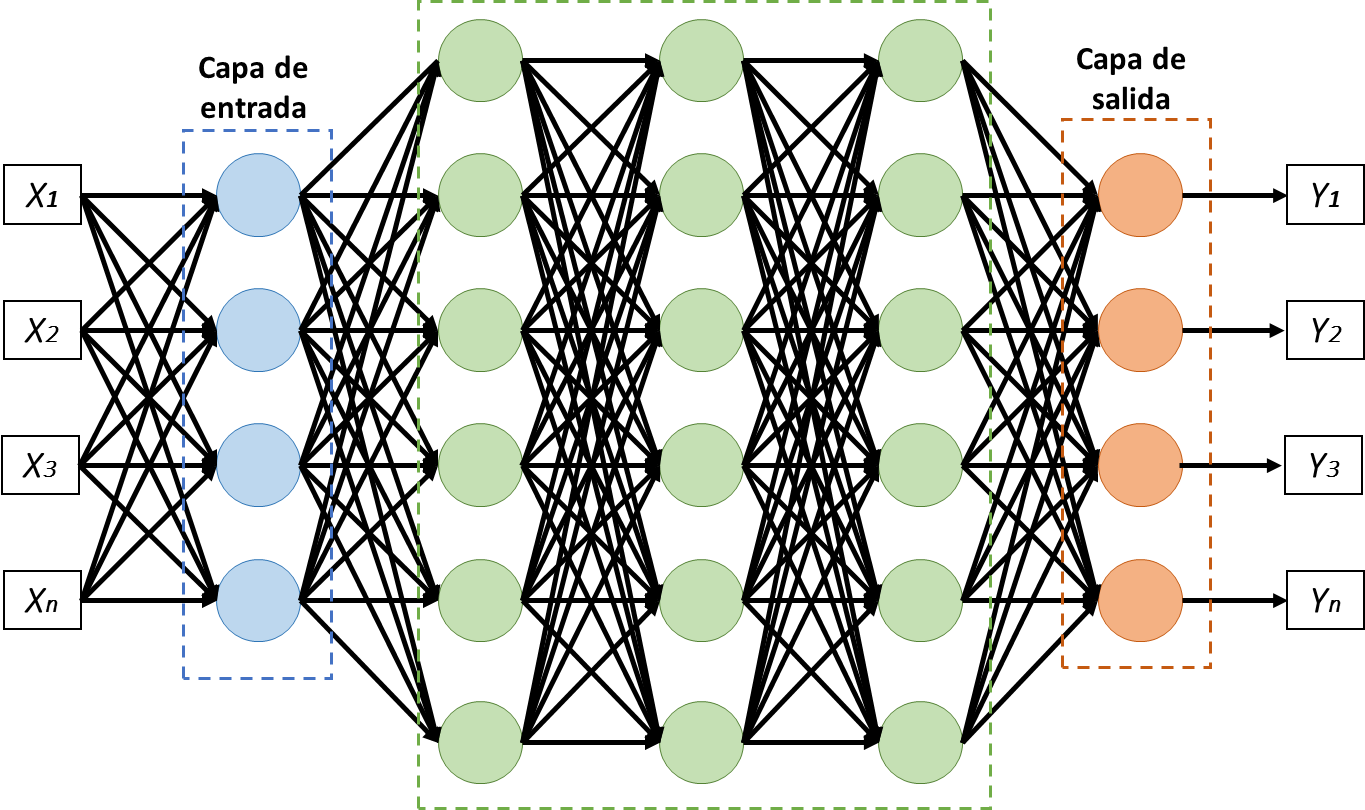
\includegraphics[scale=0.6]{ANN.png} 
            \caption{Estructura de la red neuronal artificial. \label{Fig:ANN}}
        \end{figure}

\noindent{\textbf{Anexo B.}}

\begin{figure}[h]
            \centering
            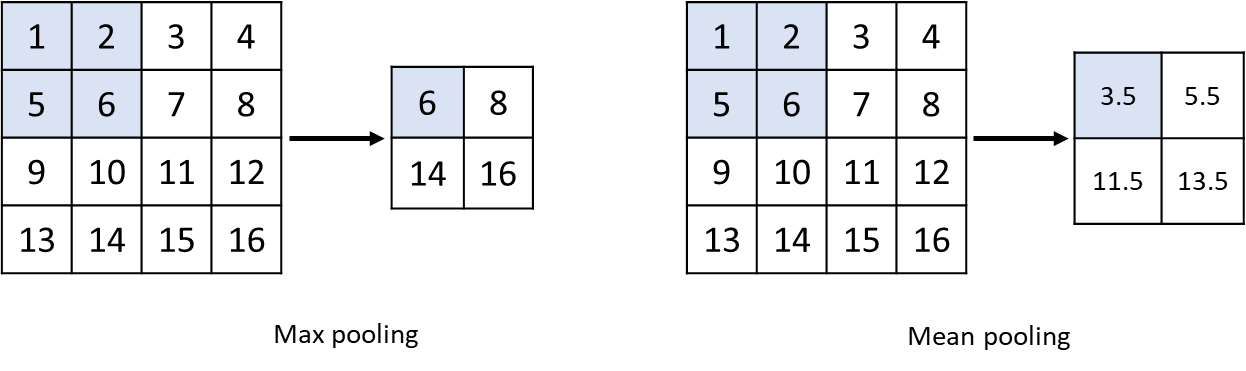
\includegraphics[scale=0.6]{Pooling.png} 
            \caption{Diagrama esquemático de agrupación máxima y agrupación media. \label{Fig:pool}}
        \end{figure}

\newpage

        
\noindent{\textbf{Anexo C.}}
\begin{figure}[H]
            \centering
            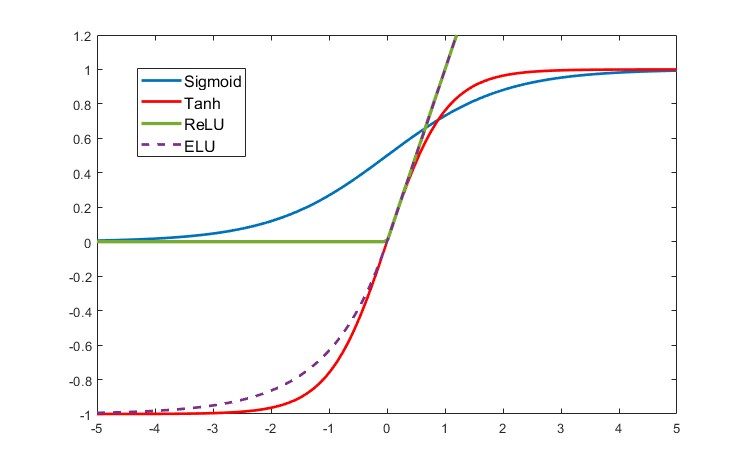
\includegraphics[width=0.8\linewidth]{Out-Actfuntions.jpg}
            \caption{Gráfico de las funciones sigmoidea, tangente hiperbólica, ReLU y ELU.}
            \label{fig:plotSIG-TANG-ReLU-ELU}
        \end{figure}

\noindent{\textbf{Anexo D.}}

    \begin{table}[H]
            \caption{Base de datos de entrenamiento en artículos basados en imágenes TC.\label{tab:TCDatabase}}
            \begin{tabular}{p{6.5cm} p{4cm}  p{4cm}}
            \hline
            \bf{Categoría} & \bf{Nombre de la base de datos} & \bf{Referencia} \\
            \hline
            Tomografías computarizadas de cáncer de pulmón con delineación manual & \href{https://www.cancerimagingarchive.net/collection/nsclc-radiomics/}{NSCLC-Radiomics} & \cite{Woo2021} \\
            \hline
            Tomografías computarizadas de cáncer de pulmón tratadas con anti-PD1 & \href{https://www.cancerimagingarchive.net/collection/anti-pd-1_lung/}{Anti-PD-1Lung} & \cite{Jiang2019} \\
            \hline
            Tomografías computarizadas con nódulos etiquetados & \href{https://luna16.grand-challenge.org/Data/}{Lung Nodule Analysis 2016 (LUNA16)} & \cite{Alakwaa2017,Salama2021,V2023} \\
            \hline
            Tomografías computarizadas con nódulos pulmonares, tumores hepáticos y ganglios linfáticos agrandados marcados & \href{https://nihcc.app.box.com/v/DeepLesion}{DeepLesion} & \cite{Tang2018,Xie2021} \\
            \hline
            Tomografías computarizadas con cáncer de pulmón marcado & \href{https://www.cancerimagingarchive.net/collection/lidc-idri/}{LIDC-IDRI} & \cite{Liu2018,Yang2021,Dutande2021,Aversano2022,V2023,Wu2023} \\
            \hline
            Tomografías computarizadas con nódulos marcados &\href{https://www.cancerimagingarchive.net/analysis-result/qin-lungct-seg/}{QIN-LungCT-Seg}& \cite{Tan2021,Woo2021}\\
            \hline
            Tomografías computarizadas con nódulos marcados & \href{https://www.cancerimagingarchive.net/collection/lidc-idri/}{RIDER Lung CT} & \cite{Cifci2022,Woo2021} \\
            \hline
            \end{tabular}
    \end{table}

    \begin{table}[H]
            \caption{Base de datos de entrenamiento en artículos basados en imágenes PET.\label{tab:PETDatabase}}
            \begin{tabular}{p{6.5cm} p{3cm} p{5cm}}
            \hline
            \bf{Categoría} & \bf{Nombre de la base de datos} & \bf{Referencia} \\
            \hline
            Exploraciones PET/CT con diagnóstico de cáncer de pulmón etiquetado & \href{https://www.cancerimagingarchive.net/collection/lung-pet-ct-dx/}{Lung-PET-CT-Dx} & \cite{Protonotarios2022,Lei2022,Xia2023} \\
            \hline
            PET/CT preentrenado & ImageNet & \cite{Li2024} \\
            \hline
            Exploraciones PET o PET/CT con diagnóstico de cáncer de pulmón etiquetado & Private & \cite{Zhang2019,Chen2022,Fruh2021,Theophraste2018,Zhao2018,Leung2020,Park2022,Yu2023,Amyar2022} \\
            \hline
            \end{tabular}
    \end{table}

        
        
\noindent{\textbf{Anexo E.}}

    \begin{figure}[H]
        \centering
        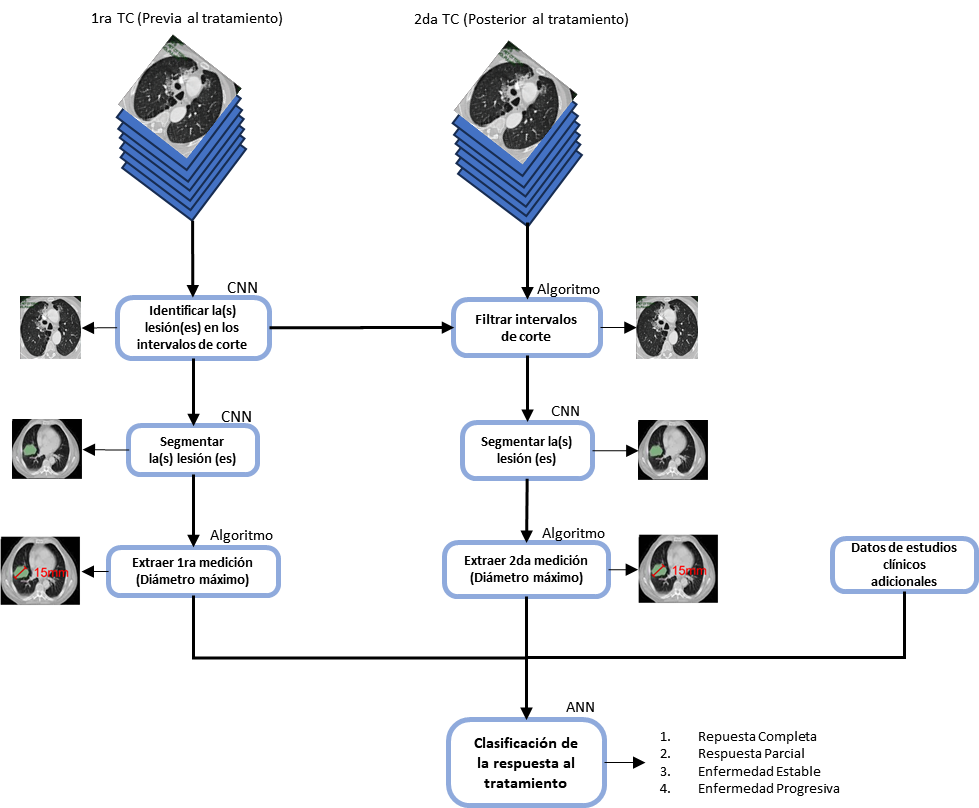
\includegraphics[width=15 cm]{SecuentialStepsEvaluation-Diagram-DL.png}
        \caption {Metodología general para la evaluación de tratamientos asistida por DL.\label{fig:SSE}}
    \end{figure}


\noindent{\textbf{Anexo F.}}

    \begin{figure}[H]
        \centering
        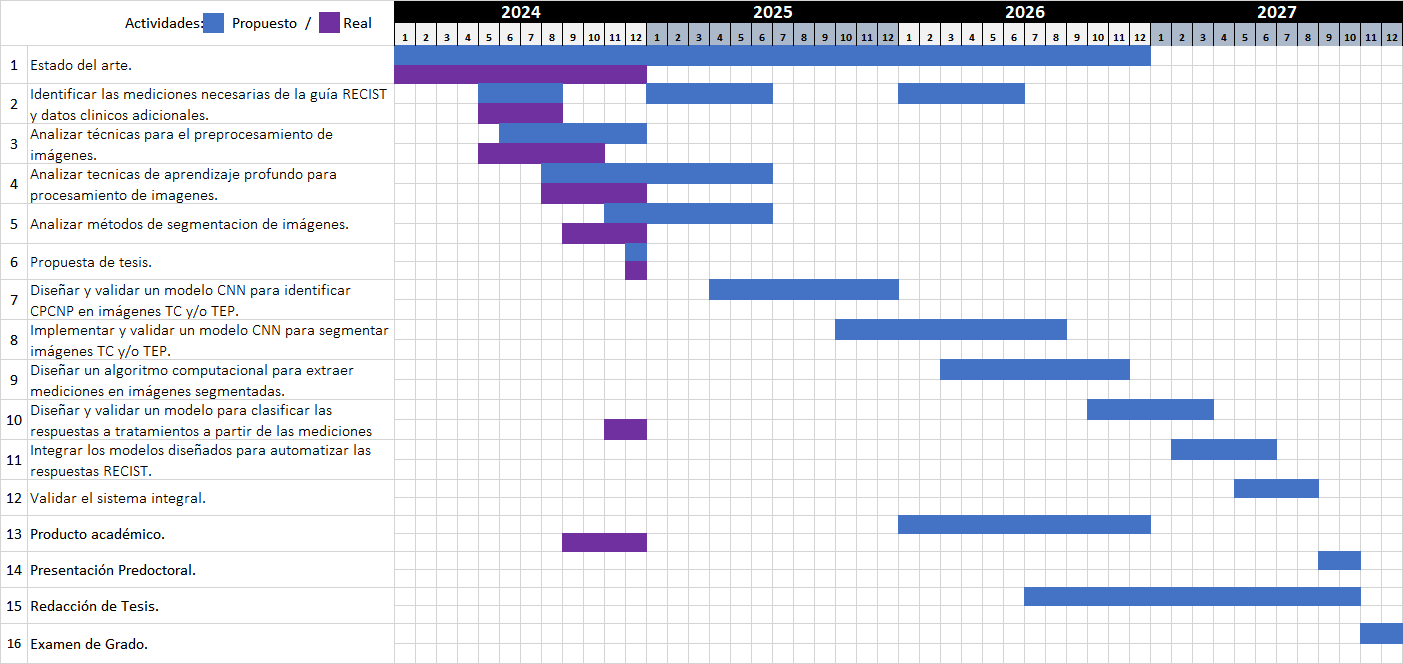
\includegraphics[width=15 cm]{cronograma.png}
        \caption {Cronograma de actividades.\label{fig:Cronograma}}
    \end{figure}

\noindent{\textbf{Anexo G.}}



\end{document}